\documentclass[a4paper]{ctexart}
\usepackage{xeCJK}
\usepackage{setspace}
\usepackage{graphicx,wrapfig}
\usepackage{fontspec,xunicode,xltxtra}
\usepackage{fancyhdr,titlesec,titletoc}
\usepackage[titletoc]{appendix}
\usepackage[top=29mm,bottom=29mm,left=31.8mm,right=31.8mm]{geometry}
\usepackage{enumerate,enumitem}
\usepackage{caption,subcaption}
\usepackage{amsmath,amssymb,bm,array}
\usepackage{cite}
\usepackage{diagbox}
\usepackage{algorithm,algorithmicx,algpseudocode}
\usepackage{multirow}
\usepackage[super]{gbt7714}
\setmainfont{Times New Roman}
\setCJKmainfont[BoldFont={Songti SC Bold}]{SimSun}
\setCJKfamilyfont{heiti}{SimHei}
\renewcommand{\heiti}{\CJKfamily{heiti}\fontspec{Times New Roman}}

\newcommand{\mycaptionfont}{\heiti\zihao{5}}
\captionsetup[figure]{name={\mycaptionfont 图},labelsep=period}
\captionsetup[table]{name={\mycaptionfont 表},labelsep=period}
\floatname{algorithm}{\mycaptionfont 算法}
\captionsetup[algorithm]{labelsep=period}
\renewcommand{\captionfont}{\mycaptionfont}
\renewcommand{\captionlabelfont}{\mycaptionfont}

\ctexset {
	section = {
		number = \arabic{section},
		format = \zihao{4}\bfseries,
	},
	subsection = {
		number = \arabic{section}.\arabic{subsection},
		format = \zihao{-4}\bfseries,
	},
	subsubsection = {
		number = \arabic{section}.\arabic{subsection}.\arabic{subsubsection},
		format = \zihao{-4}\bfseries,
	}
}
\setlist[enumerate]{itemindent=2em,listparindent=2em,leftmargin=0em,label=\arabic*、}

\setlength\parskip{.5\baselineskip}
\fancypagestyle{plain}{\pagestyle{fancy}}%改变章节首页页眉
\pagestyle{fancy}
\lhead{}
\chead{视觉物联网技术实验报告}
\rhead{}
\cfoot{\thepage}

\begin{document}
\begin{titlepage}
	\begin{center}
		
\includegraphics[width=0.9\textwidth]{figure//Njust.png}\\
		\vspace{10mm}
		\textbf{\zihao{2}\kaishu{物联网工程学院}}\\[0.8cm]
		\textbf{\zihao{2}\kaishu{视觉物联网技术实验报告}}\\[3cm]
		\textbf{\zihao{2}\kaishu{实验二~静态图像分割}}\\[3cm]
		\vspace{\fill}
		\setlength{\extrarowheight}{3mm}
		{\songti\zihao{3}
			\begin{tabular}{rl}
				{\makebox[4\ccwd][s]{班\qquad 级:}} & ~\kaishu 物联1601   \\
				{\makebox[4\ccwd][s]{姓\qquad 名:}} & ~\kaishu 尹达恒     \\
				{\makebox[4\ccwd][s]{学\qquad 号:}} & ~\kaishu 1030616134 \\
				{\makebox[4\ccwd][s]{指导老师:}}    & ~\kaishu 陈莹       \\
			\end{tabular}
		}\\[2cm]
		\vspace{\fill}
		\zihao{4}
		2018\textasciitilde 2019第二学期\\
		2019年5月
	\end{center}
\end{titlepage}

\renewcommand{\baselinestretch}{1.3}
\zihao{-4}
\section{实验目的}
\begin{enumerate}[label=\arabic*、]
	\item 使学生通过实验体会一些主要的分割算法对图像处理的效果,以及各种因素对分割效果的影响;
	\item 使用 Matlab 软件进行图像的分割;
	\item 能够自行评价各主要算子在有无干扰环境下的分割性能;
	\item 能够掌握分割条件(算法中各种参数等)的选择;
	\item 完成规定图像的处理并要求正确评价处理结果,能够在算法原理层面作出合理的解释。
\end{enumerate}

\section{实验内容}
\begin{enumerate}[label=\arabic*、]
	\item 将图1-图5水表图像中的指示指针从背景中分离(指针部分显示为白色,其余部分显示为 黑色);(注:所有图采用统一代码)
	\item 利用二值形态学对分割后的二值图像进行处理以消除分割噪声;
	\item 利用MATLAB形态学算子调整分割结果;
	\item 根据分割结果给出水表读数(各位置指针所对应的单位可通过人为先验确定)。
\end{enumerate}
\begin{figure*}[htbp]
	\centering
	\begin{minipage}[t]{0.25\textwidth}
		\centering
		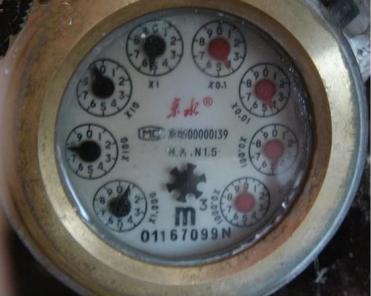
\includegraphics[width=\textwidth]{figure/img1.jpg}
		\caption{}\label{fig:1}
	\end{minipage}
	\begin{minipage}[t]{0.25\textwidth}
		\centering
		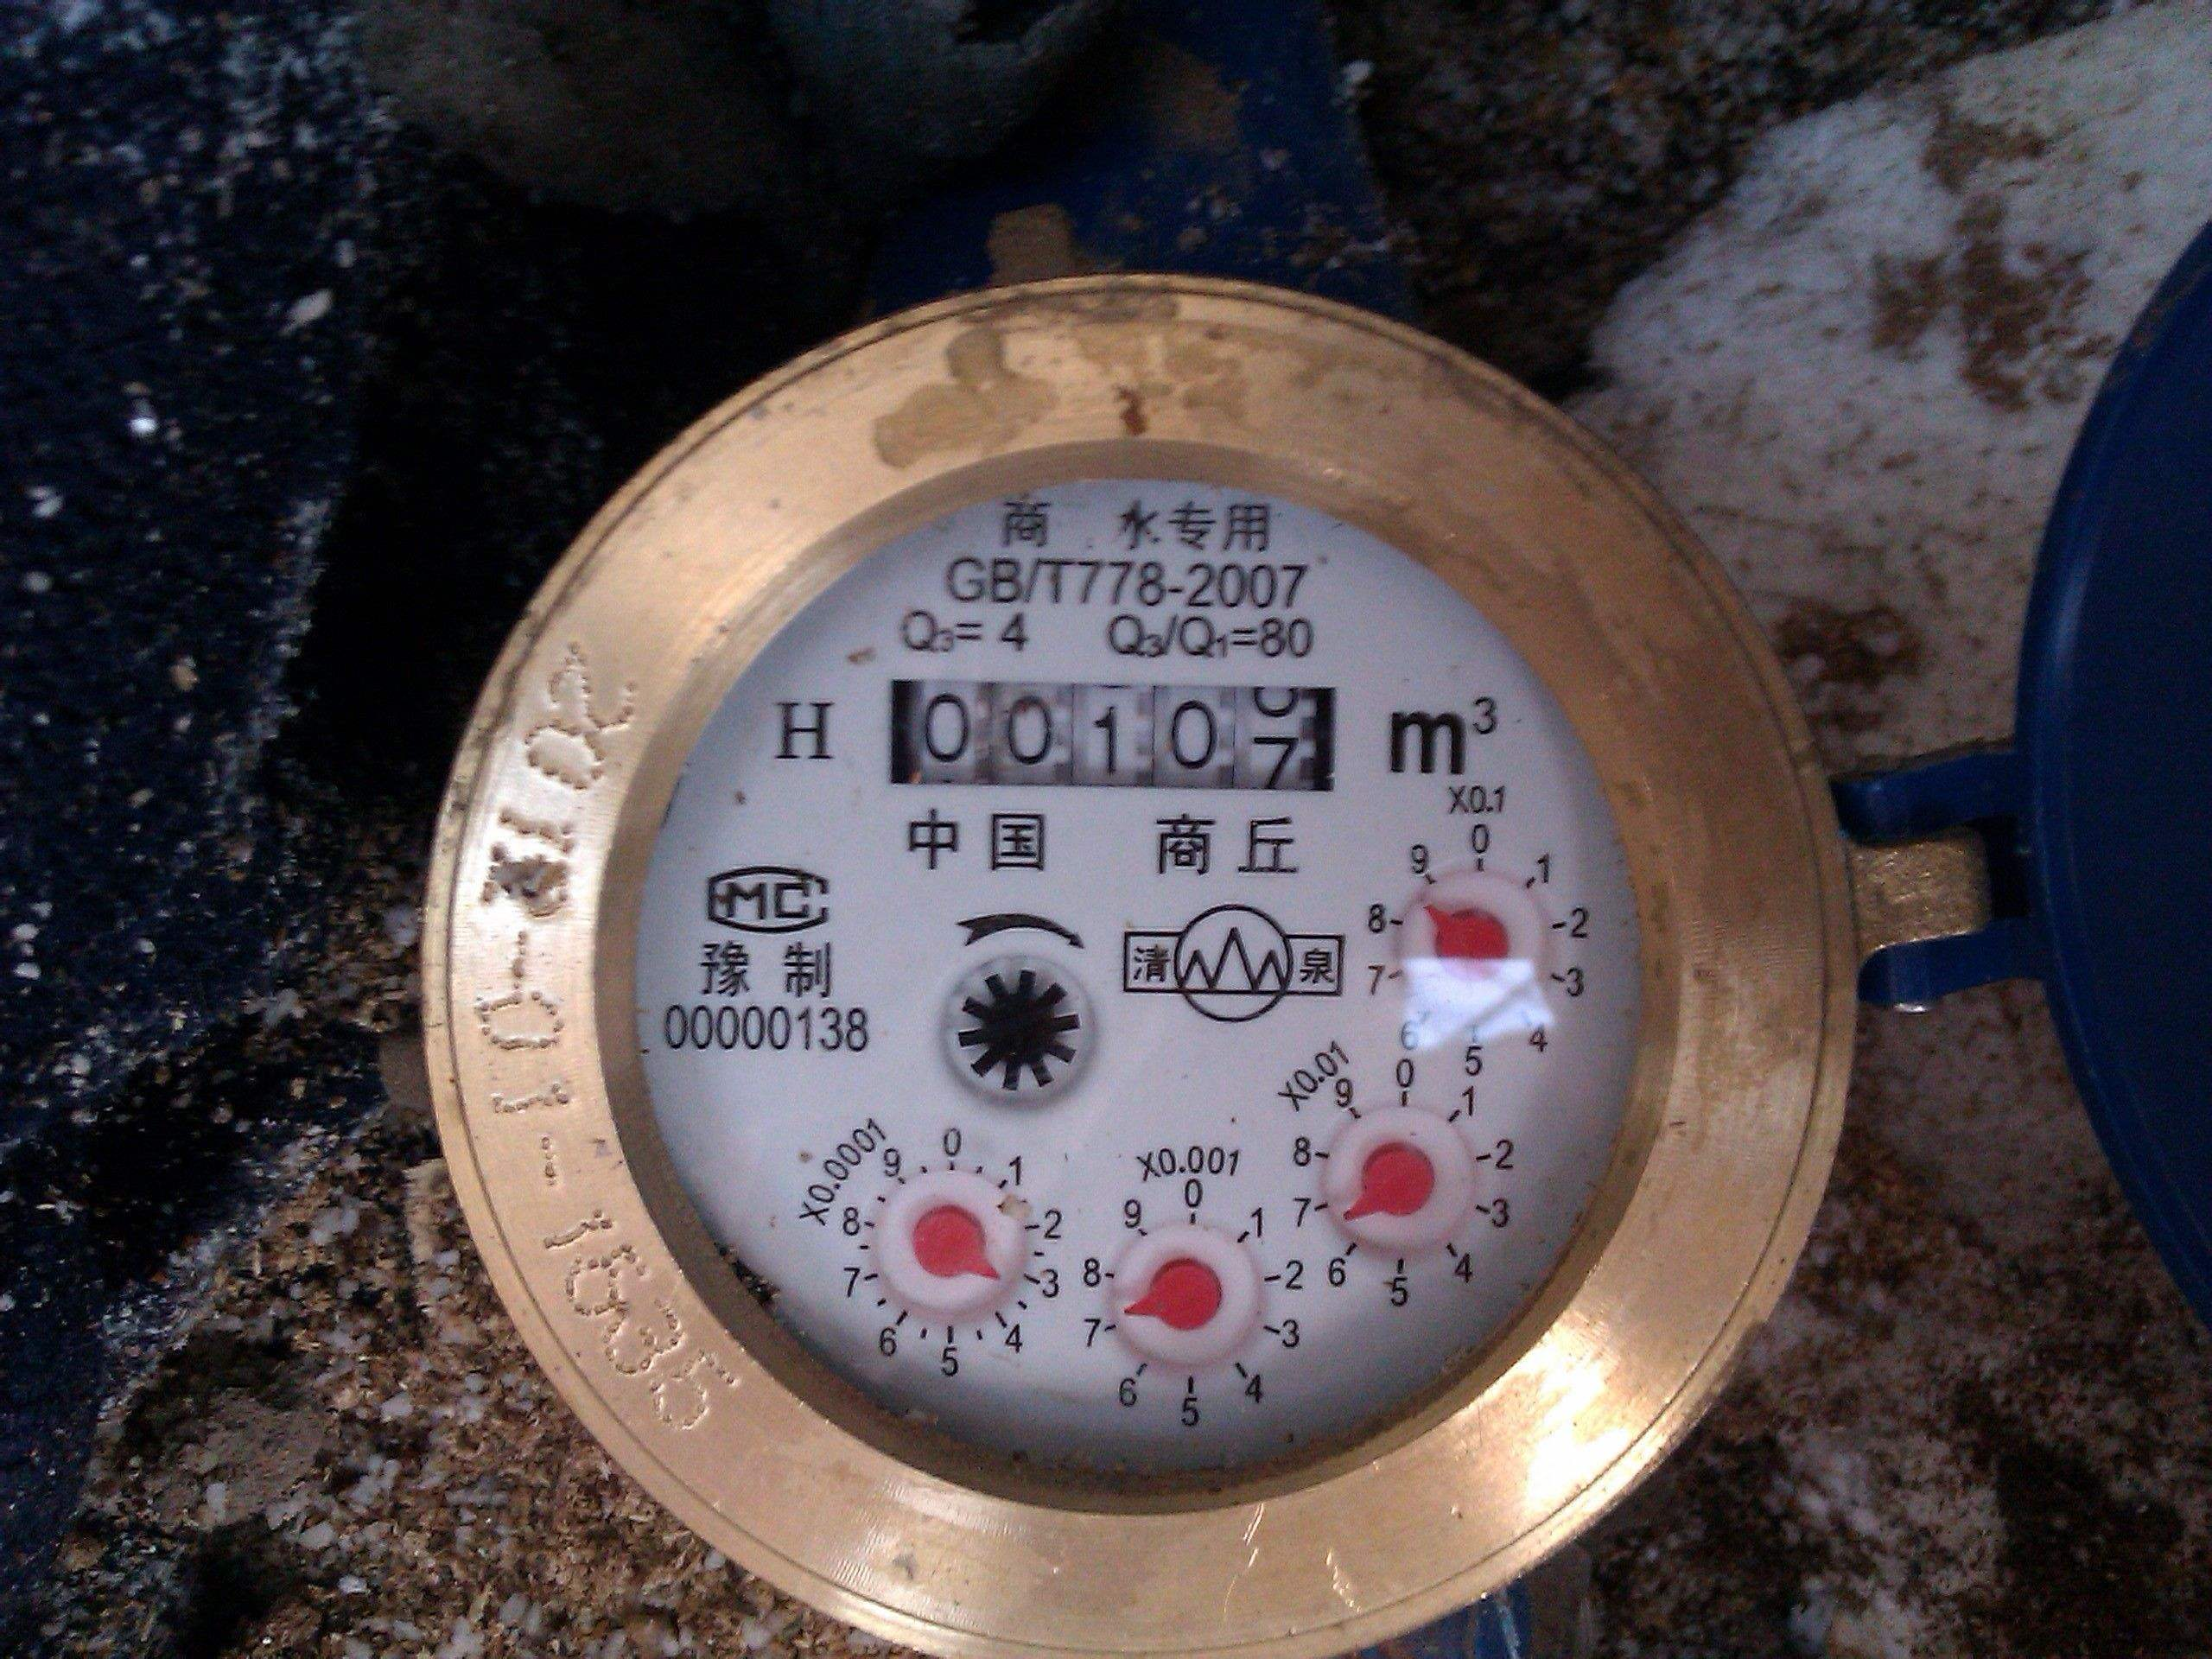
\includegraphics[width=\textwidth]{figure/img2.jpg}
		\caption{}\label{fig:2}
	\end{minipage}\\
	\begin{minipage}[t]{0.25\textwidth}
		\centering
		
\includegraphics[width=\textwidth]{figure/img3.jpg}
		\caption{}\label{fig:3}
	\end{minipage}
	\begin{minipage}[t]{0.25\textwidth}
		\centering
		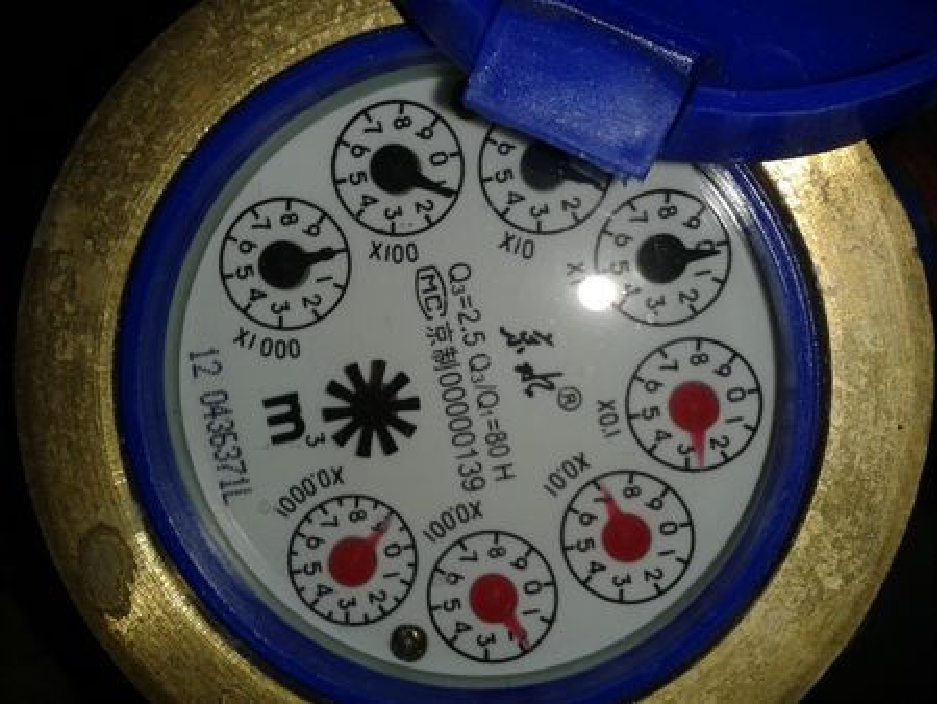
\includegraphics[width=\textwidth]{figure/img4.pdf}
		\caption{}\label{fig:4}
	\end{minipage}
	\begin{minipage}[t]{0.25\textwidth}
		\centering
		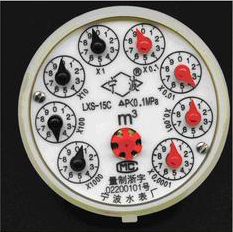
\includegraphics[width=\textwidth]{figure/img5.jpg}
		\caption{}\label{fig:5}
	\end{minipage}
\end{figure*}

\section{实验步骤}
\subsection{图像增强}\label{sec:色彩增强}
由图1-图5水表图像中可以看出,图1-图4中的目标区域(指针)和周边图像的对比度不明显,不利于目标区域的提取,因此需要对图像进行颜色特征的增强以增大目标区域与其他区域的差别从而便于目标区域的提取。
\subsubsection{直方图均衡化}
直方图均衡化的基本思想是把原始图的直方图变换为均匀分布的形式,这样就增加了象素灰度值的动态范围从而可达到增强图像整体对比度的效果。如果直接对彩色图像R,G,B三通道分别均衡化后再合并,极容易出现颜色不均、失真等问题,所以,一般会将RGB图像转换到YCrCb空间,对Y通道进行均衡化(Y通道代表亮度成分)。

本文采用Opencv3中的直方图均衡化函数equalizeHist对转换到YCrCb空间的实验图像进行直方图均衡化,形成程序文件“equalizeHist.py”对图像进行处理,均衡化效果如图\ref{fig:直方图均衡化}。

\begin{figure}[htbp]
	\centering
	\begin{minipage}[t]{0.25\textwidth}
		\centering
		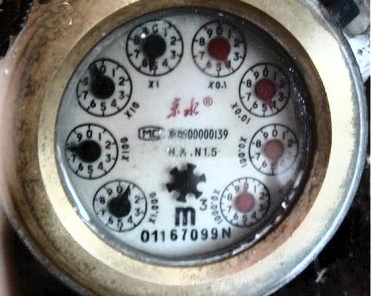
\includegraphics[width=\textwidth]{figure/equalizeHist/img1.jpg}
	\end{minipage}
	\begin{minipage}[t]{0.25\textwidth}
		\centering
		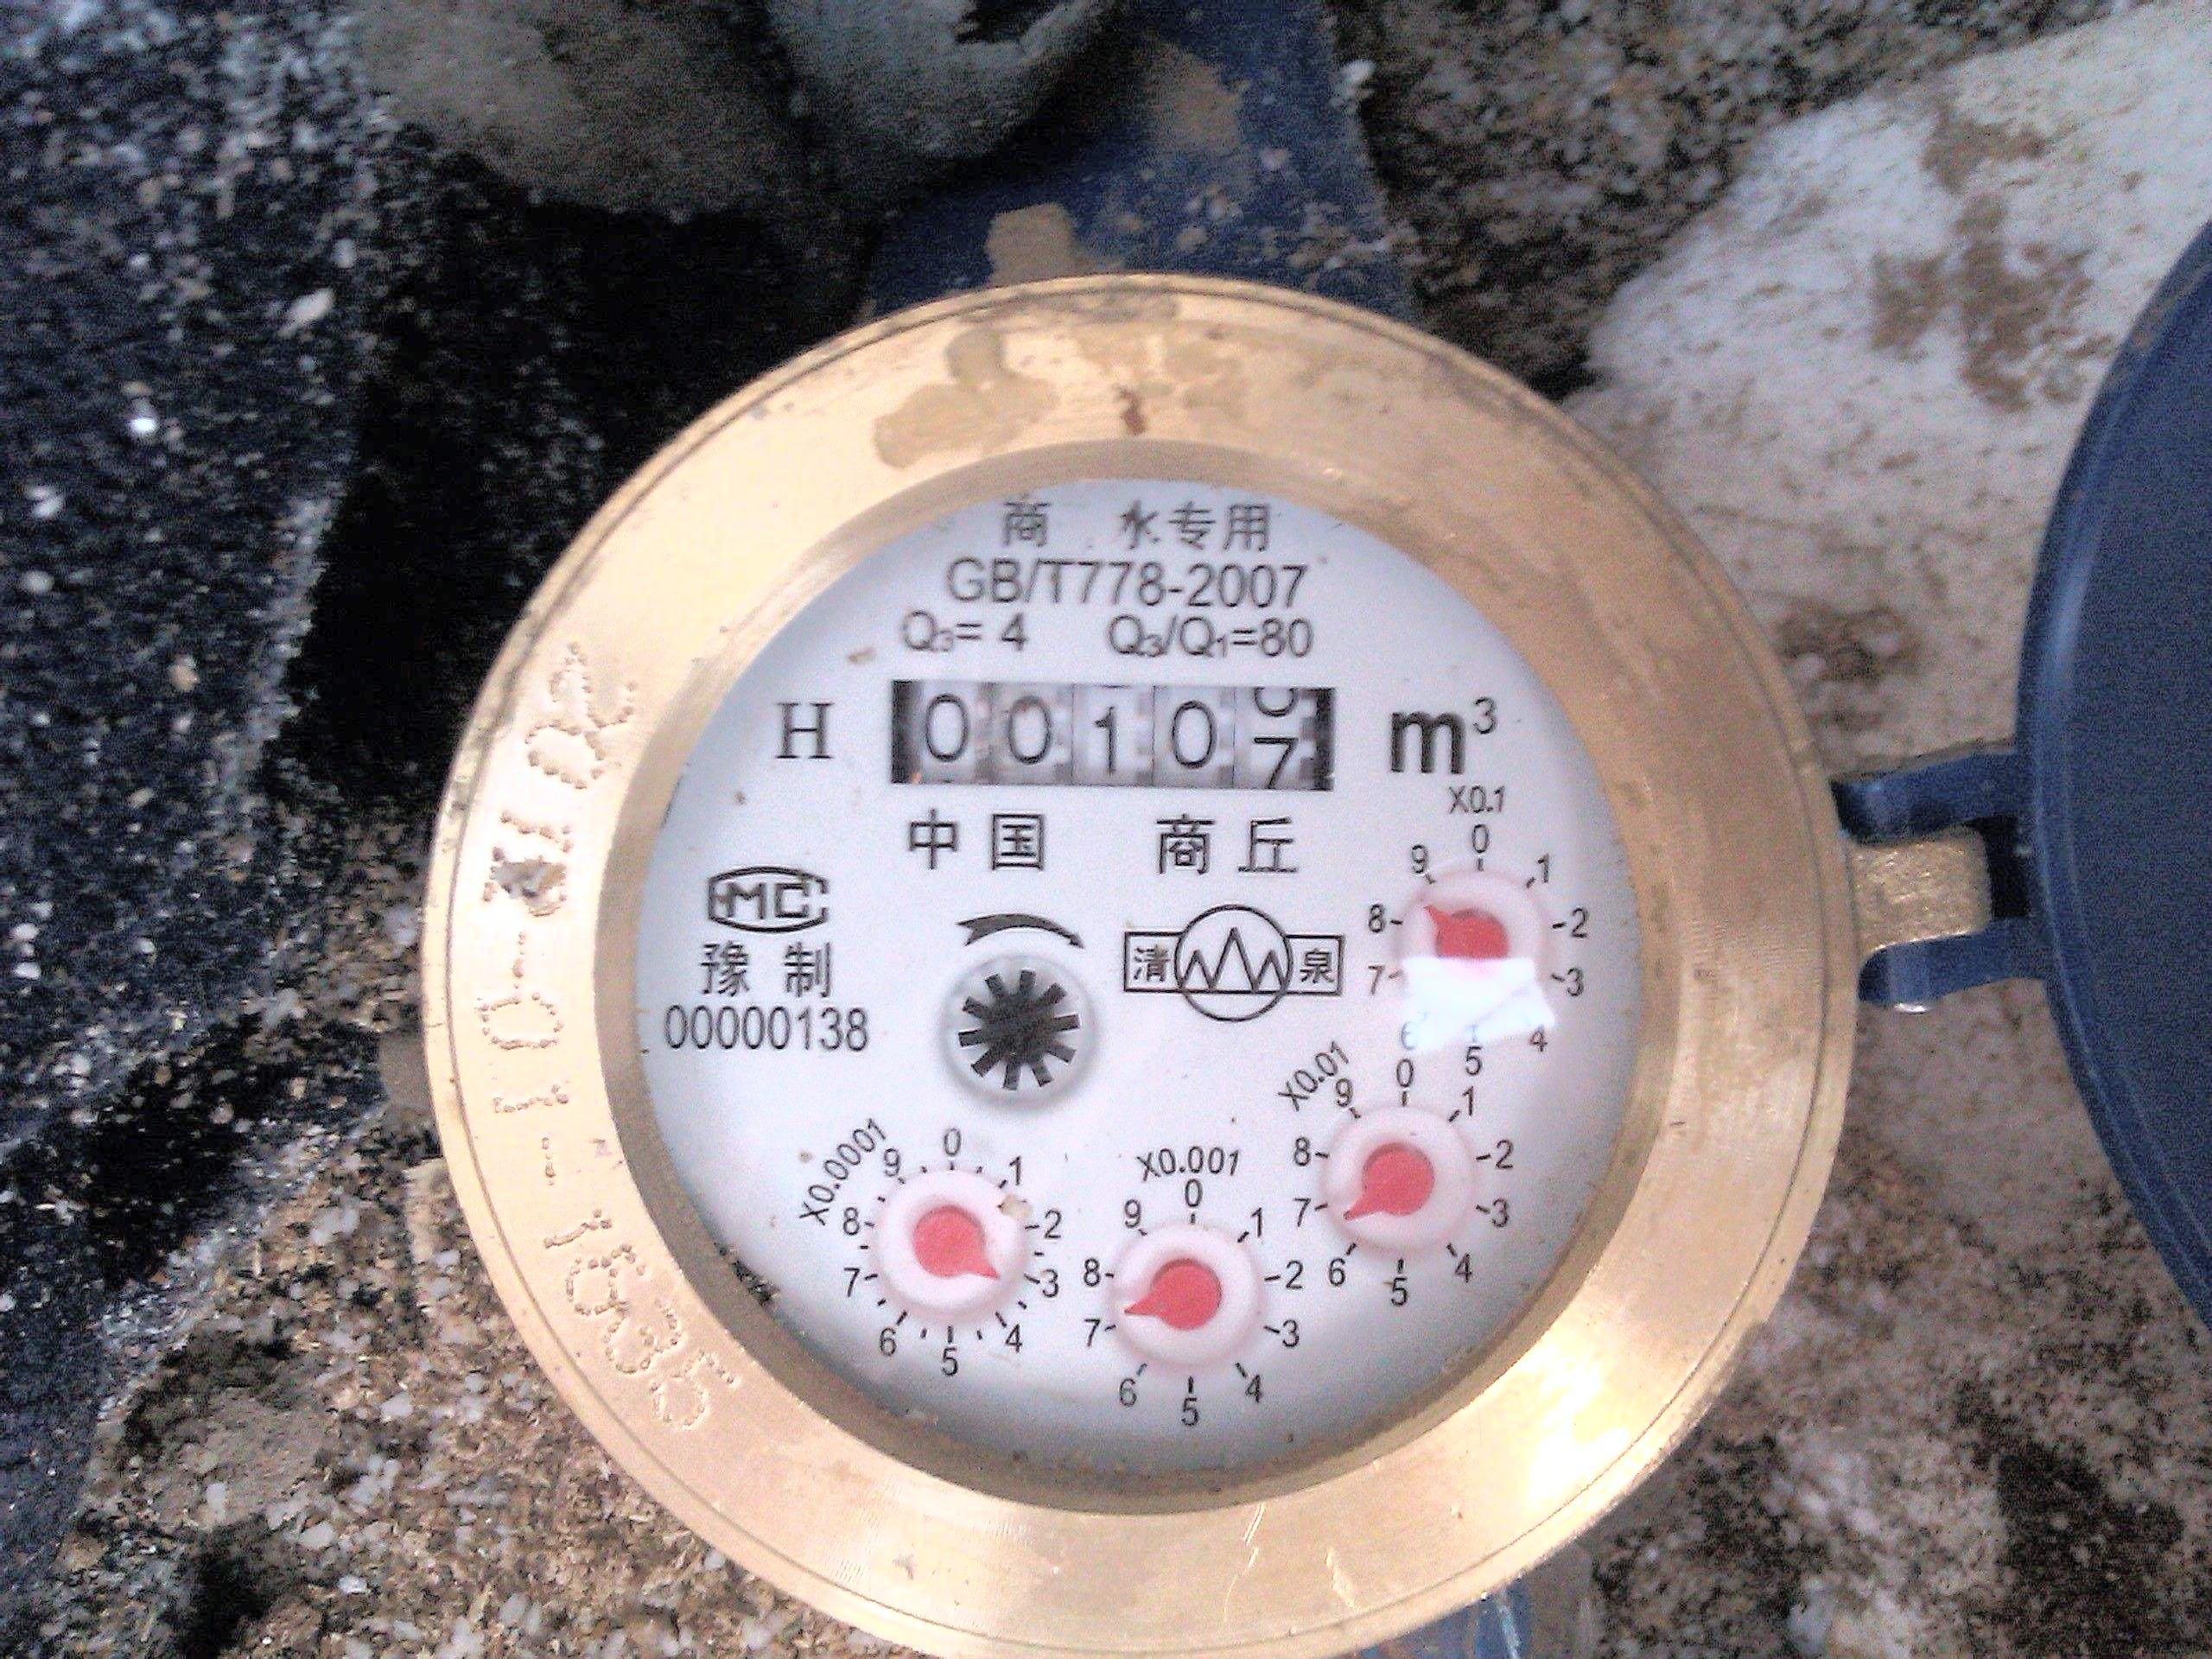
\includegraphics[width=\textwidth]{figure/equalizeHist/img2.jpg}
	\end{minipage}\\
	\begin{minipage}[t]{0.25\textwidth}
		\centering
		
\includegraphics[width=\textwidth]{figure/equalizeHist/img3.jpg}
	\end{minipage}
	\begin{minipage}[t]{0.25\textwidth}
		\centering
		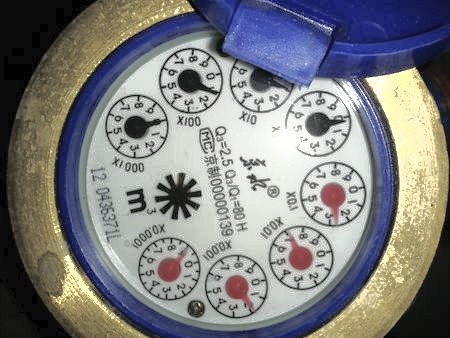
\includegraphics[width=\textwidth]{figure/equalizeHist/img4.jpg}
	\end{minipage}
	\begin{minipage}[t]{0.25\textwidth}
		\centering
		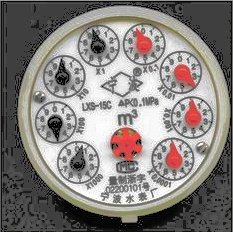
\includegraphics[width=\textwidth]{figure/equalizeHist/img5.jpg}
	\end{minipage}
	\caption{直方图均衡化处理结果}\label{fig:直方图均衡化}
\end{figure}


\subsubsection{Retinex色彩增强}
Retinex色彩理论由Edwin Land于1977年\cite{land1971lightness}首次提出,这种增强算法首先依据像素的R、G、B分量将输入的彩色图像被分解成为三幅图像,代表场景中波长不同(长波、中波和短波)的反射光的强度;分别计算长波、中波和短波波段内像素间的相对明暗关系,进而确定每个像素的色彩。最后,将Retinex色度空间内的色彩线性映射到RGB空间,获得经过增强的图像。通过这种方法所获得的图像具有色彩逼真度、动态范围大的特点。目前常用的Retinex色彩增强算法主要是具有色彩恢复的多尺度Retinex算法(Multi-Scale Retinex with Color Restoration, MSRCR)\cite{rahman1996multiscale},该算法在多尺度下对图像进行Retinex色彩增强,并加入了色彩恢复因子C来调节由于图像局部区域对比度增强而导致颜色失真的缺陷,解决了一般Retinex色彩增强因为增加了噪声,而使得图像的局部细节色彩失真的问题。

本文采用Matlab编写MSRCR程序,设置尺度数量100,对比度参数2.5,形成函数程序文件“msrcr.m”和脚本“msrcr\_run.m”对图像进行处理,色彩增强效果如图\ref{fig:MSRCR}。

\begin{figure}[htbp]
	\centering
	\begin{minipage}[t]{0.25\textwidth}
		\centering
		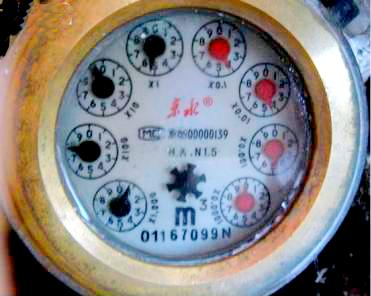
\includegraphics[width=\textwidth]{figure/msrcr/img1.jpg}
	\end{minipage}
	\begin{minipage}[t]{0.25\textwidth}
		\centering
		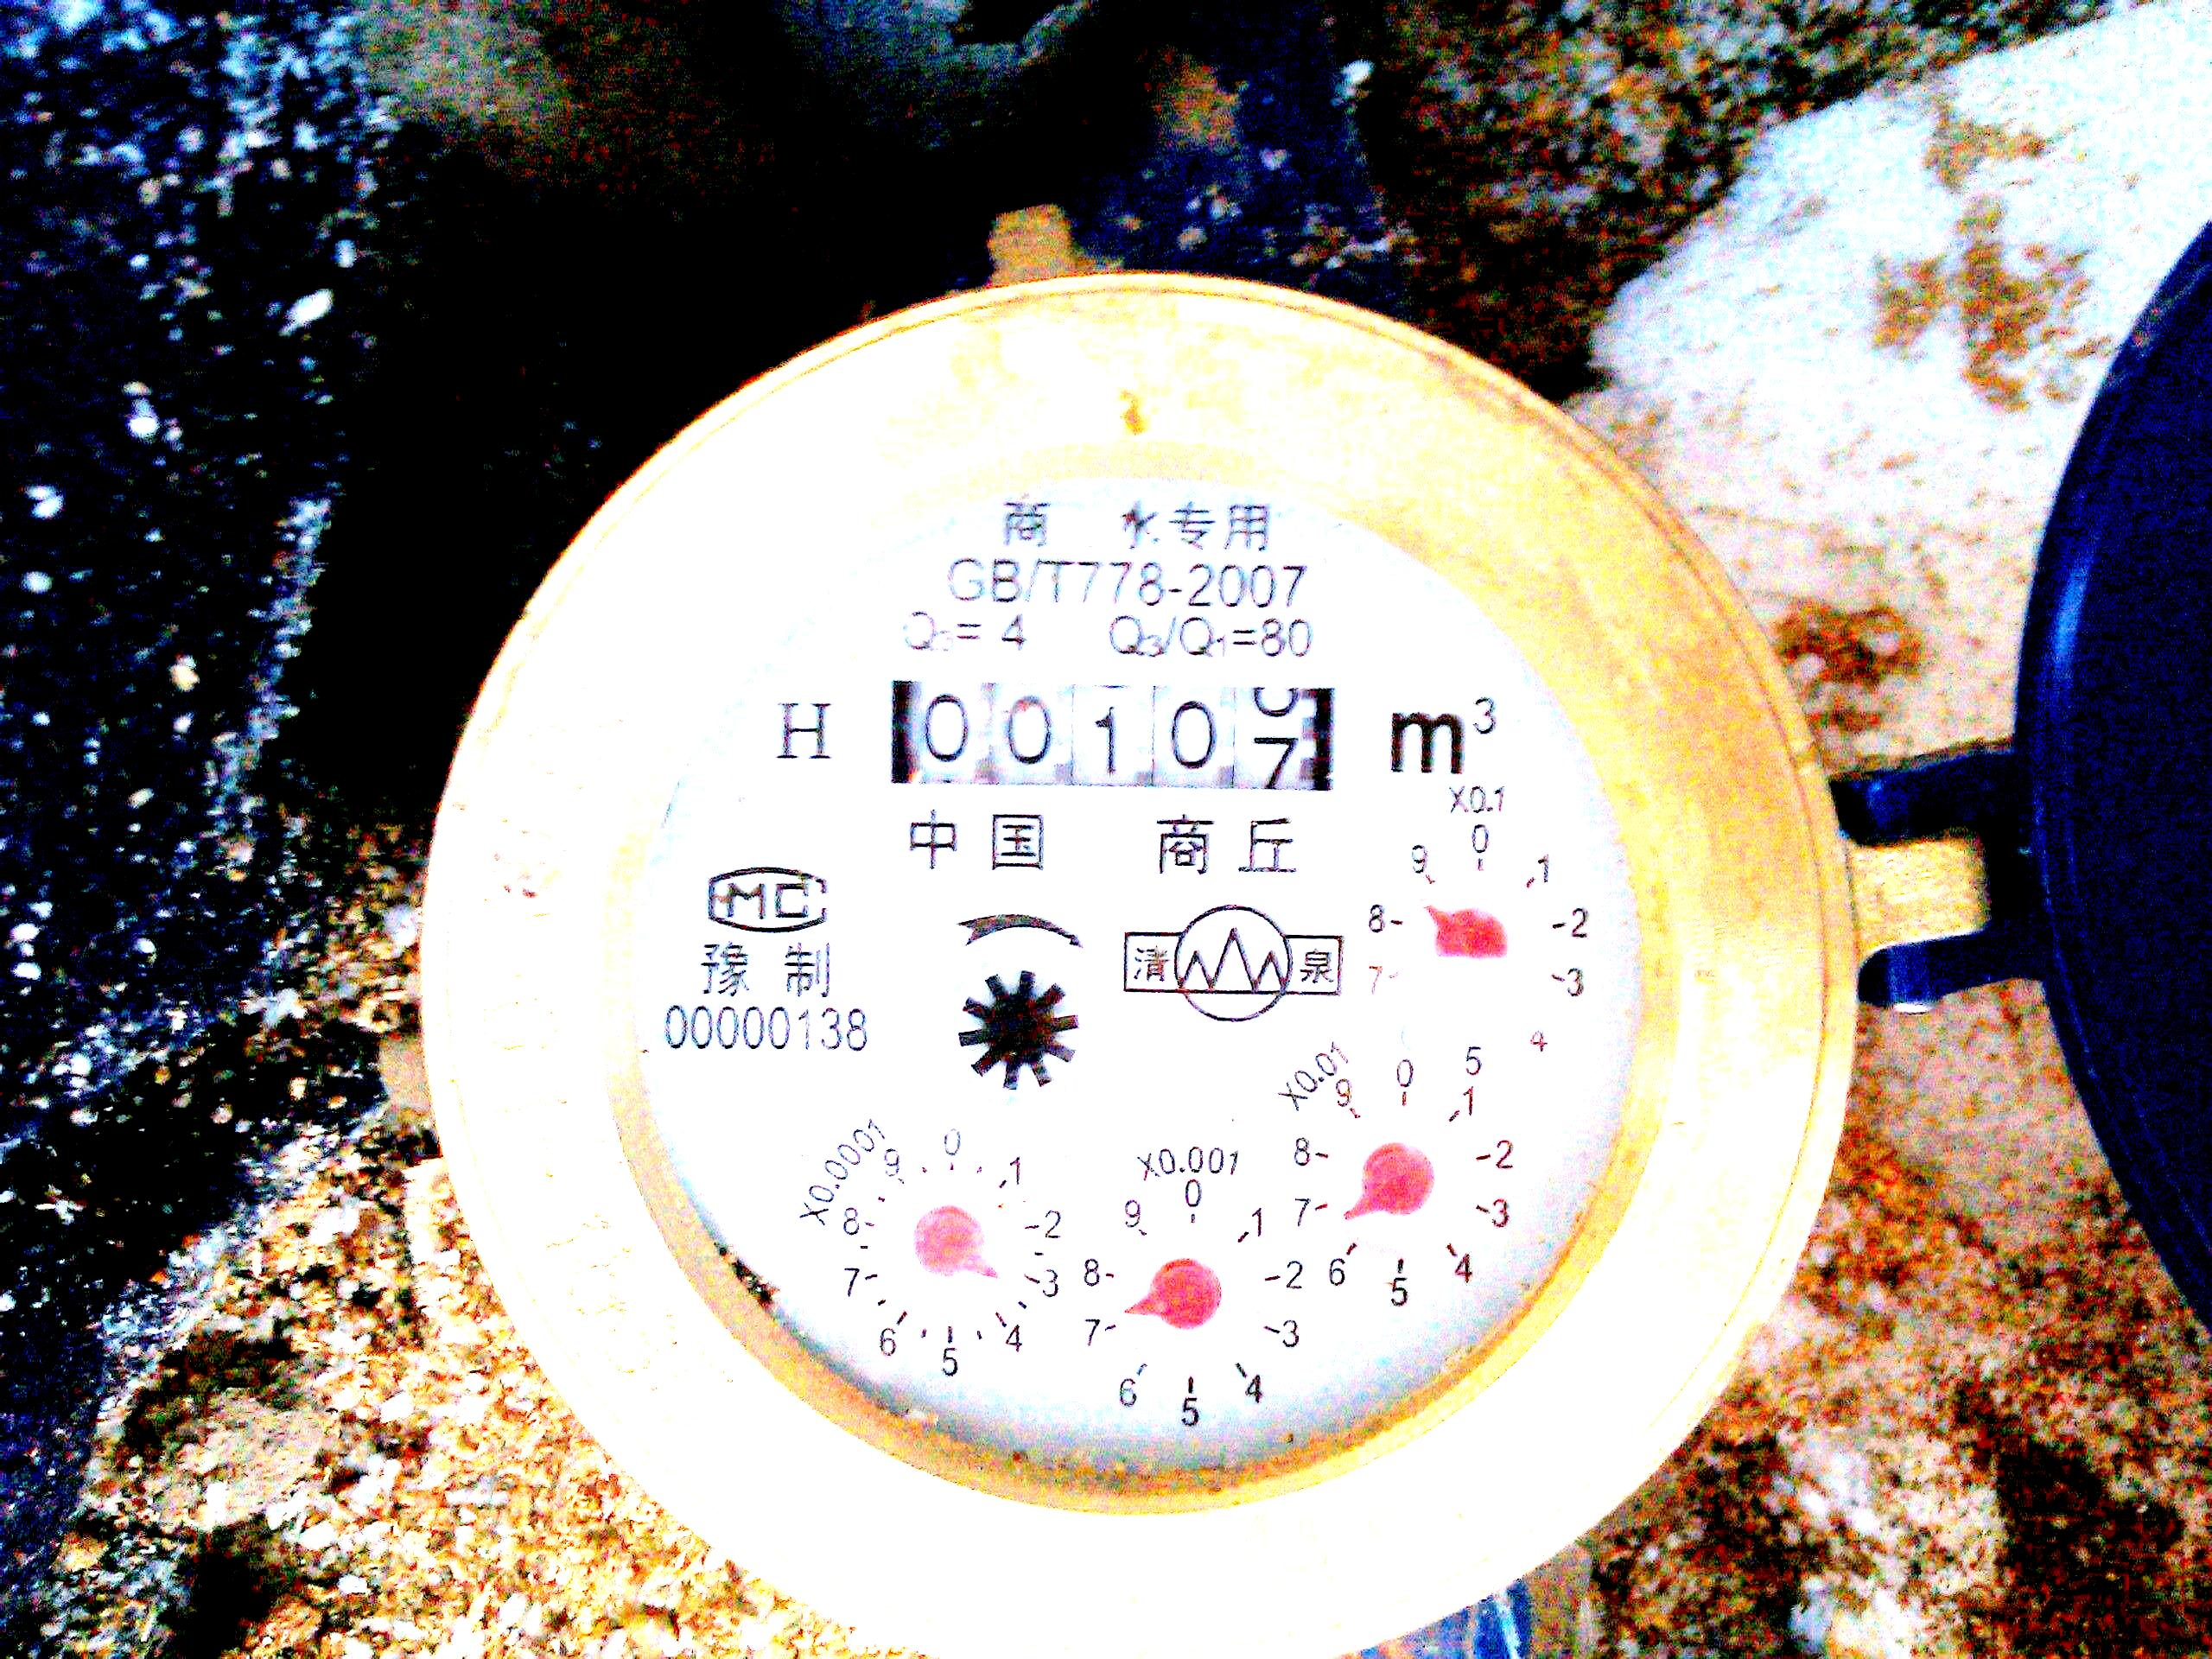
\includegraphics[width=\textwidth]{figure/msrcr/img2.jpg}
	\end{minipage}\\
	\begin{minipage}[t]{0.25\textwidth}
		\centering
		
\includegraphics[width=\textwidth]{figure/msrcr/img3.jpg}
	\end{minipage}
	\begin{minipage}[t]{0.25\textwidth}
		\centering
		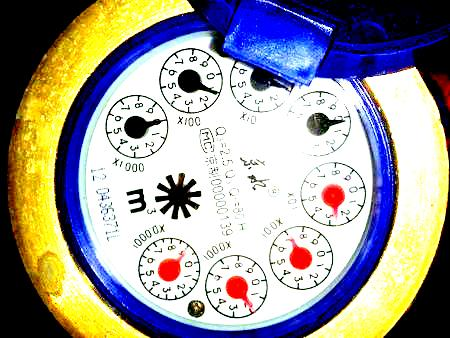
\includegraphics[width=\textwidth]{figure/msrcr/img4.jpg}
	\end{minipage}
	\begin{minipage}[t]{0.25\textwidth}
		\centering
		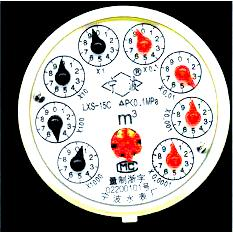
\includegraphics[width=\textwidth]{figure/msrcr/img5.jpg}
	\end{minipage}
	\caption{MSRCR处理结果}\label{fig:MSRCR}
\end{figure}

\subsection{区域提取}
当图像增强操作完成后,接下来就需要进行目标区域的提取。从结果图\ref{fig:MSRCR}和图\ref{fig:直方图均衡化}对比可以看出,MSRCR方法更加有效地突出了图像中的指针部分,因此本文选用图\ref{fig:MSRCR}中的结果进行进一步的区域提取操作。
\subsubsection{阈值化颜色范围}\label{sec:阈值化}
红色指针区域的提取可以采用基于颜色的提取方法。将MSRCR增强后的图像转化到YCbCr空间,提取Cr通道以灰度形式保存,形成“R\_channel.py”,处理结果如图\ref{fig:Cr通道}。

\begin{figure}[htbp]
	\centering
	\begin{minipage}[t]{0.25\textwidth}
		\centering
		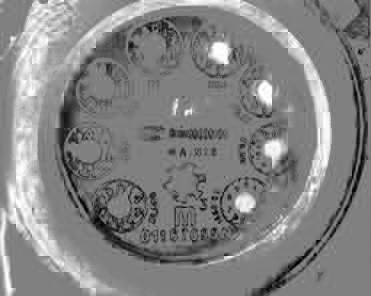
\includegraphics[width=\textwidth]{figure/R_channel/img1.jpg}
	\end{minipage}
	\begin{minipage}[t]{0.25\textwidth}
		\centering
		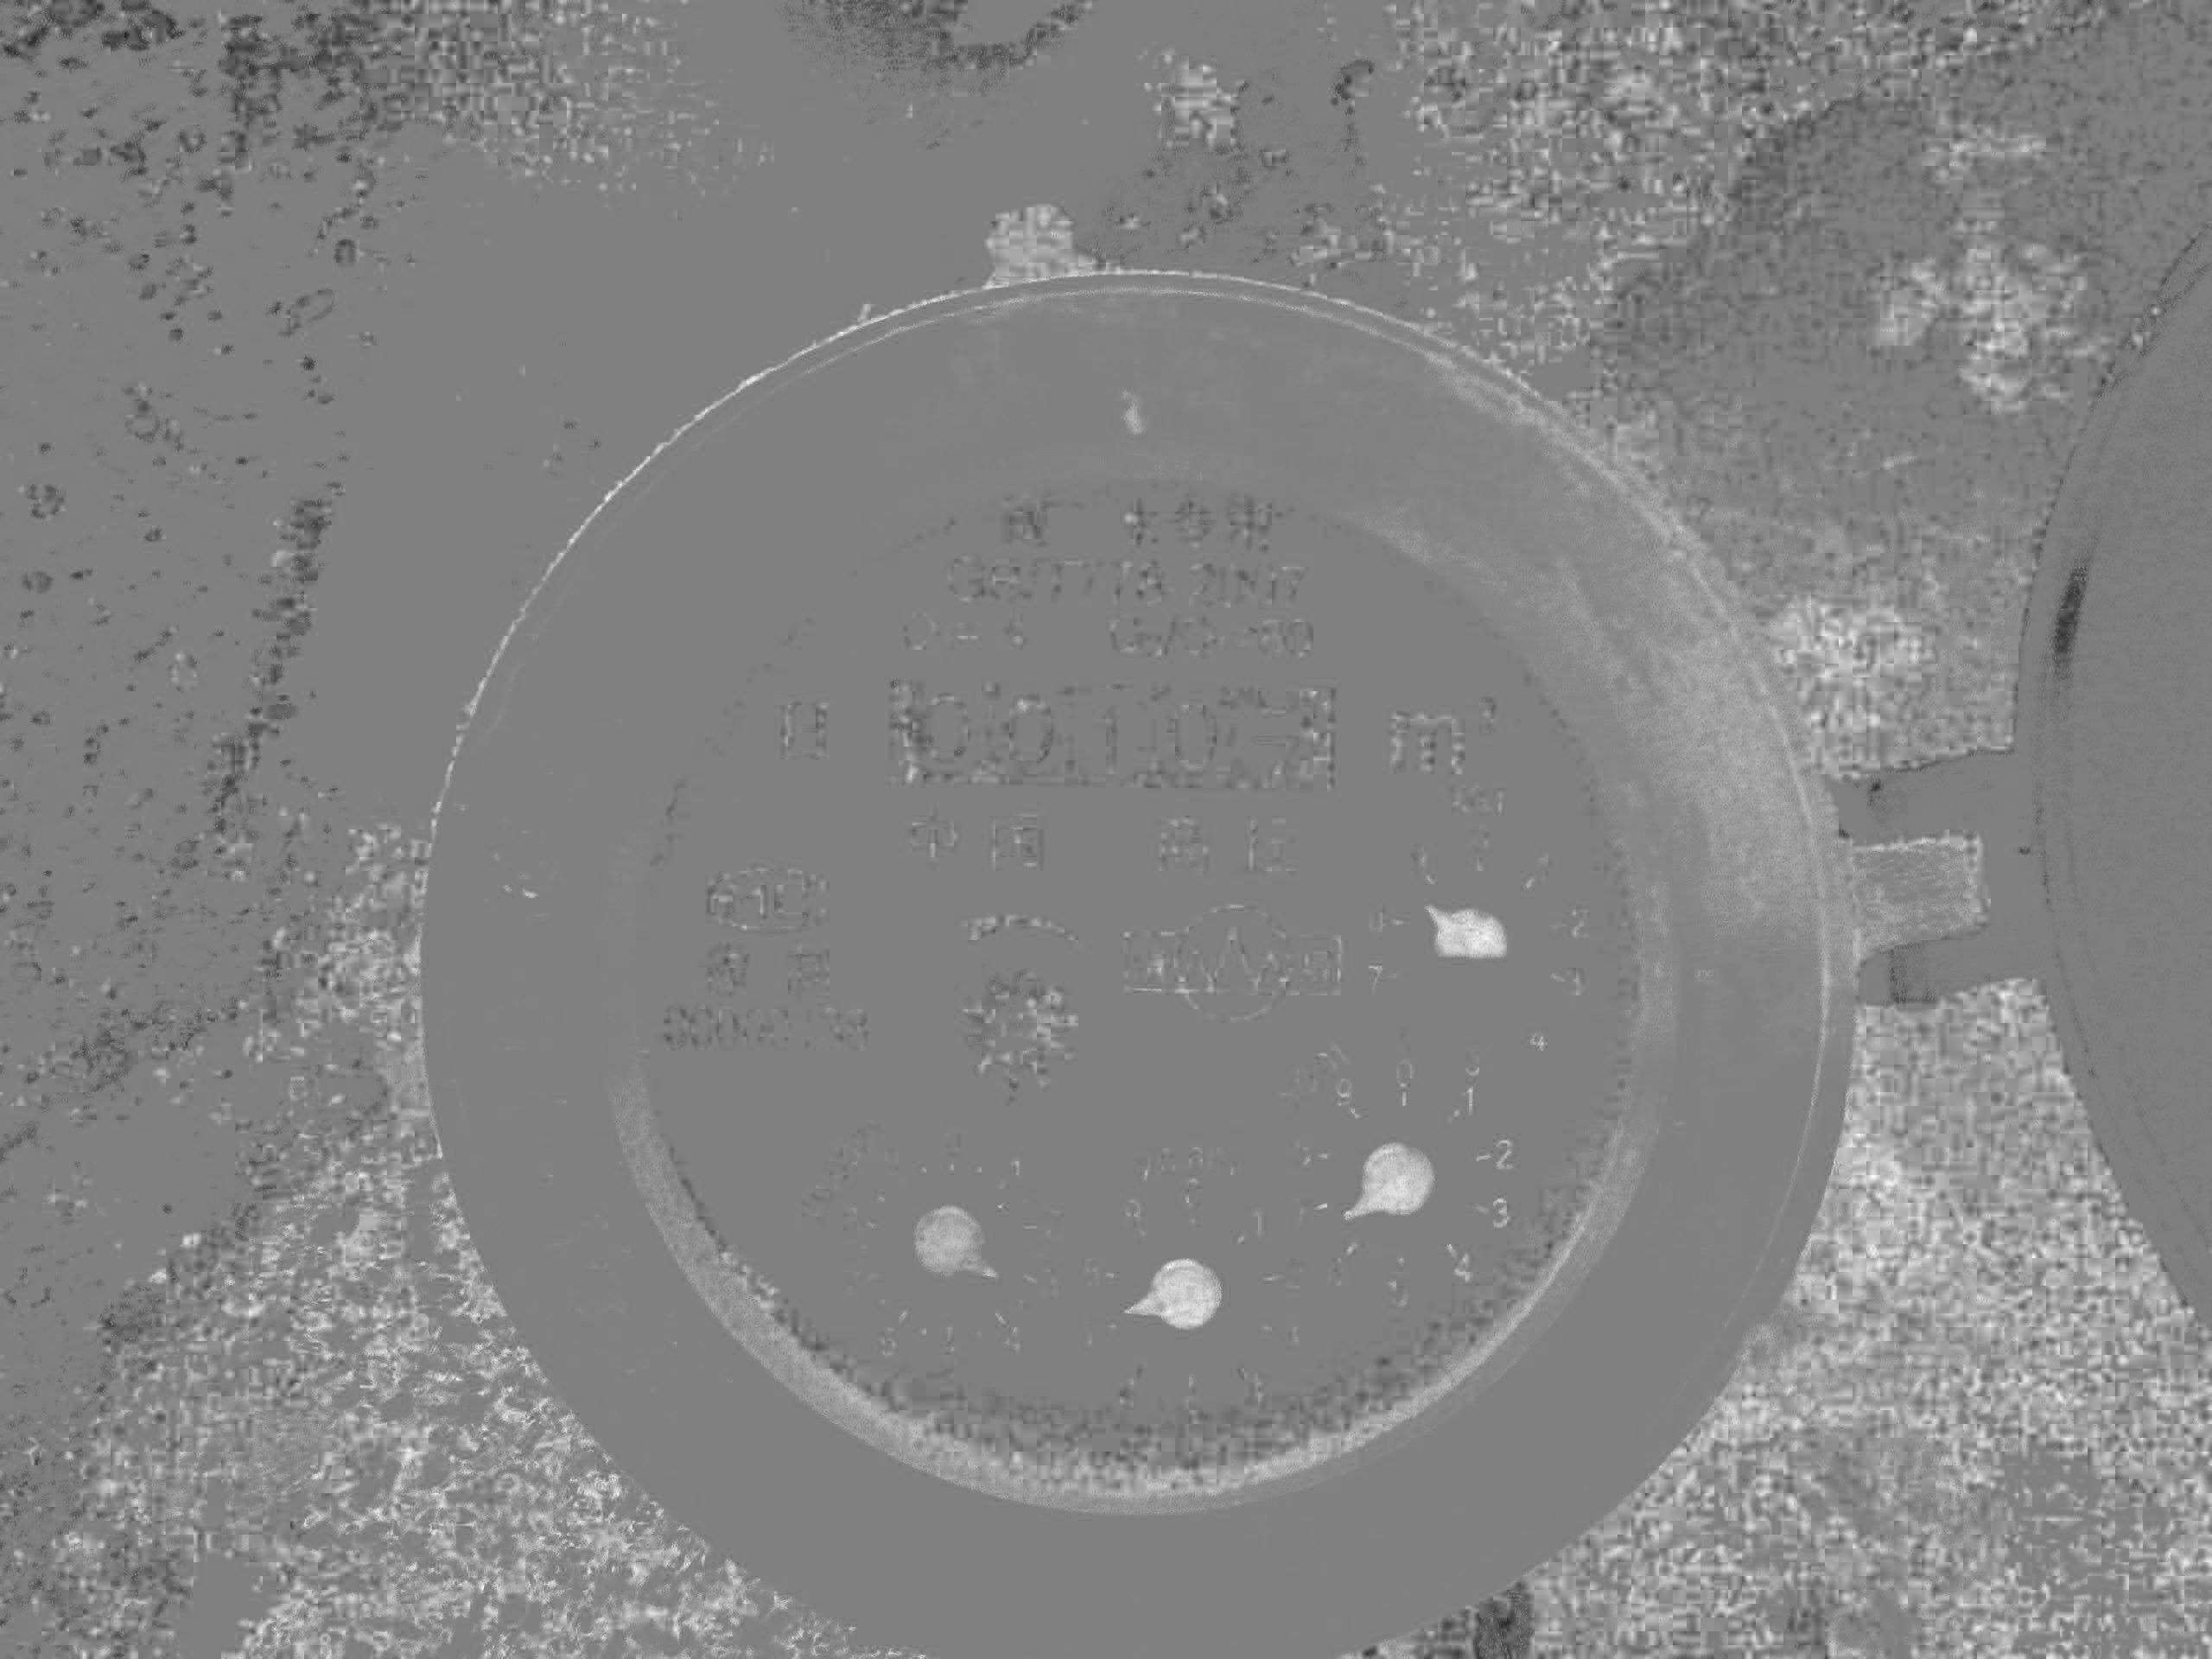
\includegraphics[width=\textwidth]{figure/R_channel/img2.jpg}
	\end{minipage}\\
	\begin{minipage}[t]{0.25\textwidth}
		\centering
		
\includegraphics[width=\textwidth]{figure/R_channel/img3.jpg}
	\end{minipage}
	\begin{minipage}[t]{0.25\textwidth}
		\centering
		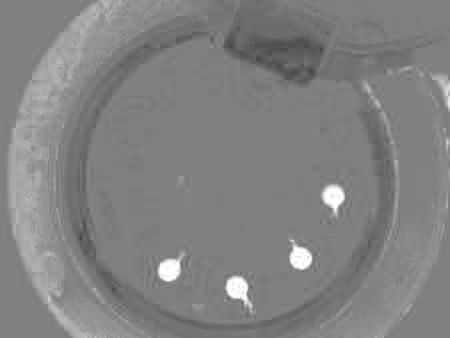
\includegraphics[width=\textwidth]{figure/R_channel/img4.jpg}
	\end{minipage}
	\begin{minipage}[t]{0.25\textwidth}
		\centering
		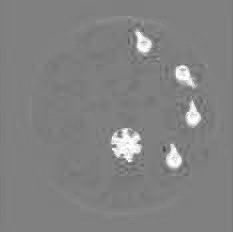
\includegraphics[width=\textwidth]{figure/R_channel/img5.jpg}
	\end{minipage}
	\caption{提取Cr通道结果}\label{fig:Cr通道}
\end{figure}

经过观察调整,可以尝试出对于5张图均有较好的色彩提取效果的阈值为150,形成程序文件“threshold.py”提取出的Cr通道进行阈值化处理,结果如图\ref{fig:阈值化}。

\begin{figure}[htbp]
	\centering
	\begin{minipage}[t]{0.25\textwidth}
		\centering
		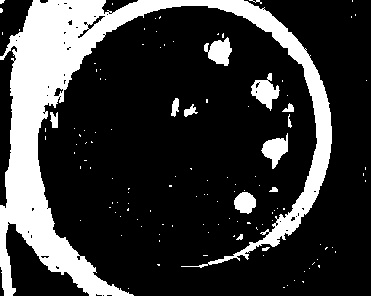
\includegraphics[width=\textwidth]{figure/threshold/img1.jpg}
	\end{minipage}
	\begin{minipage}[t]{0.25\textwidth}
		\centering
		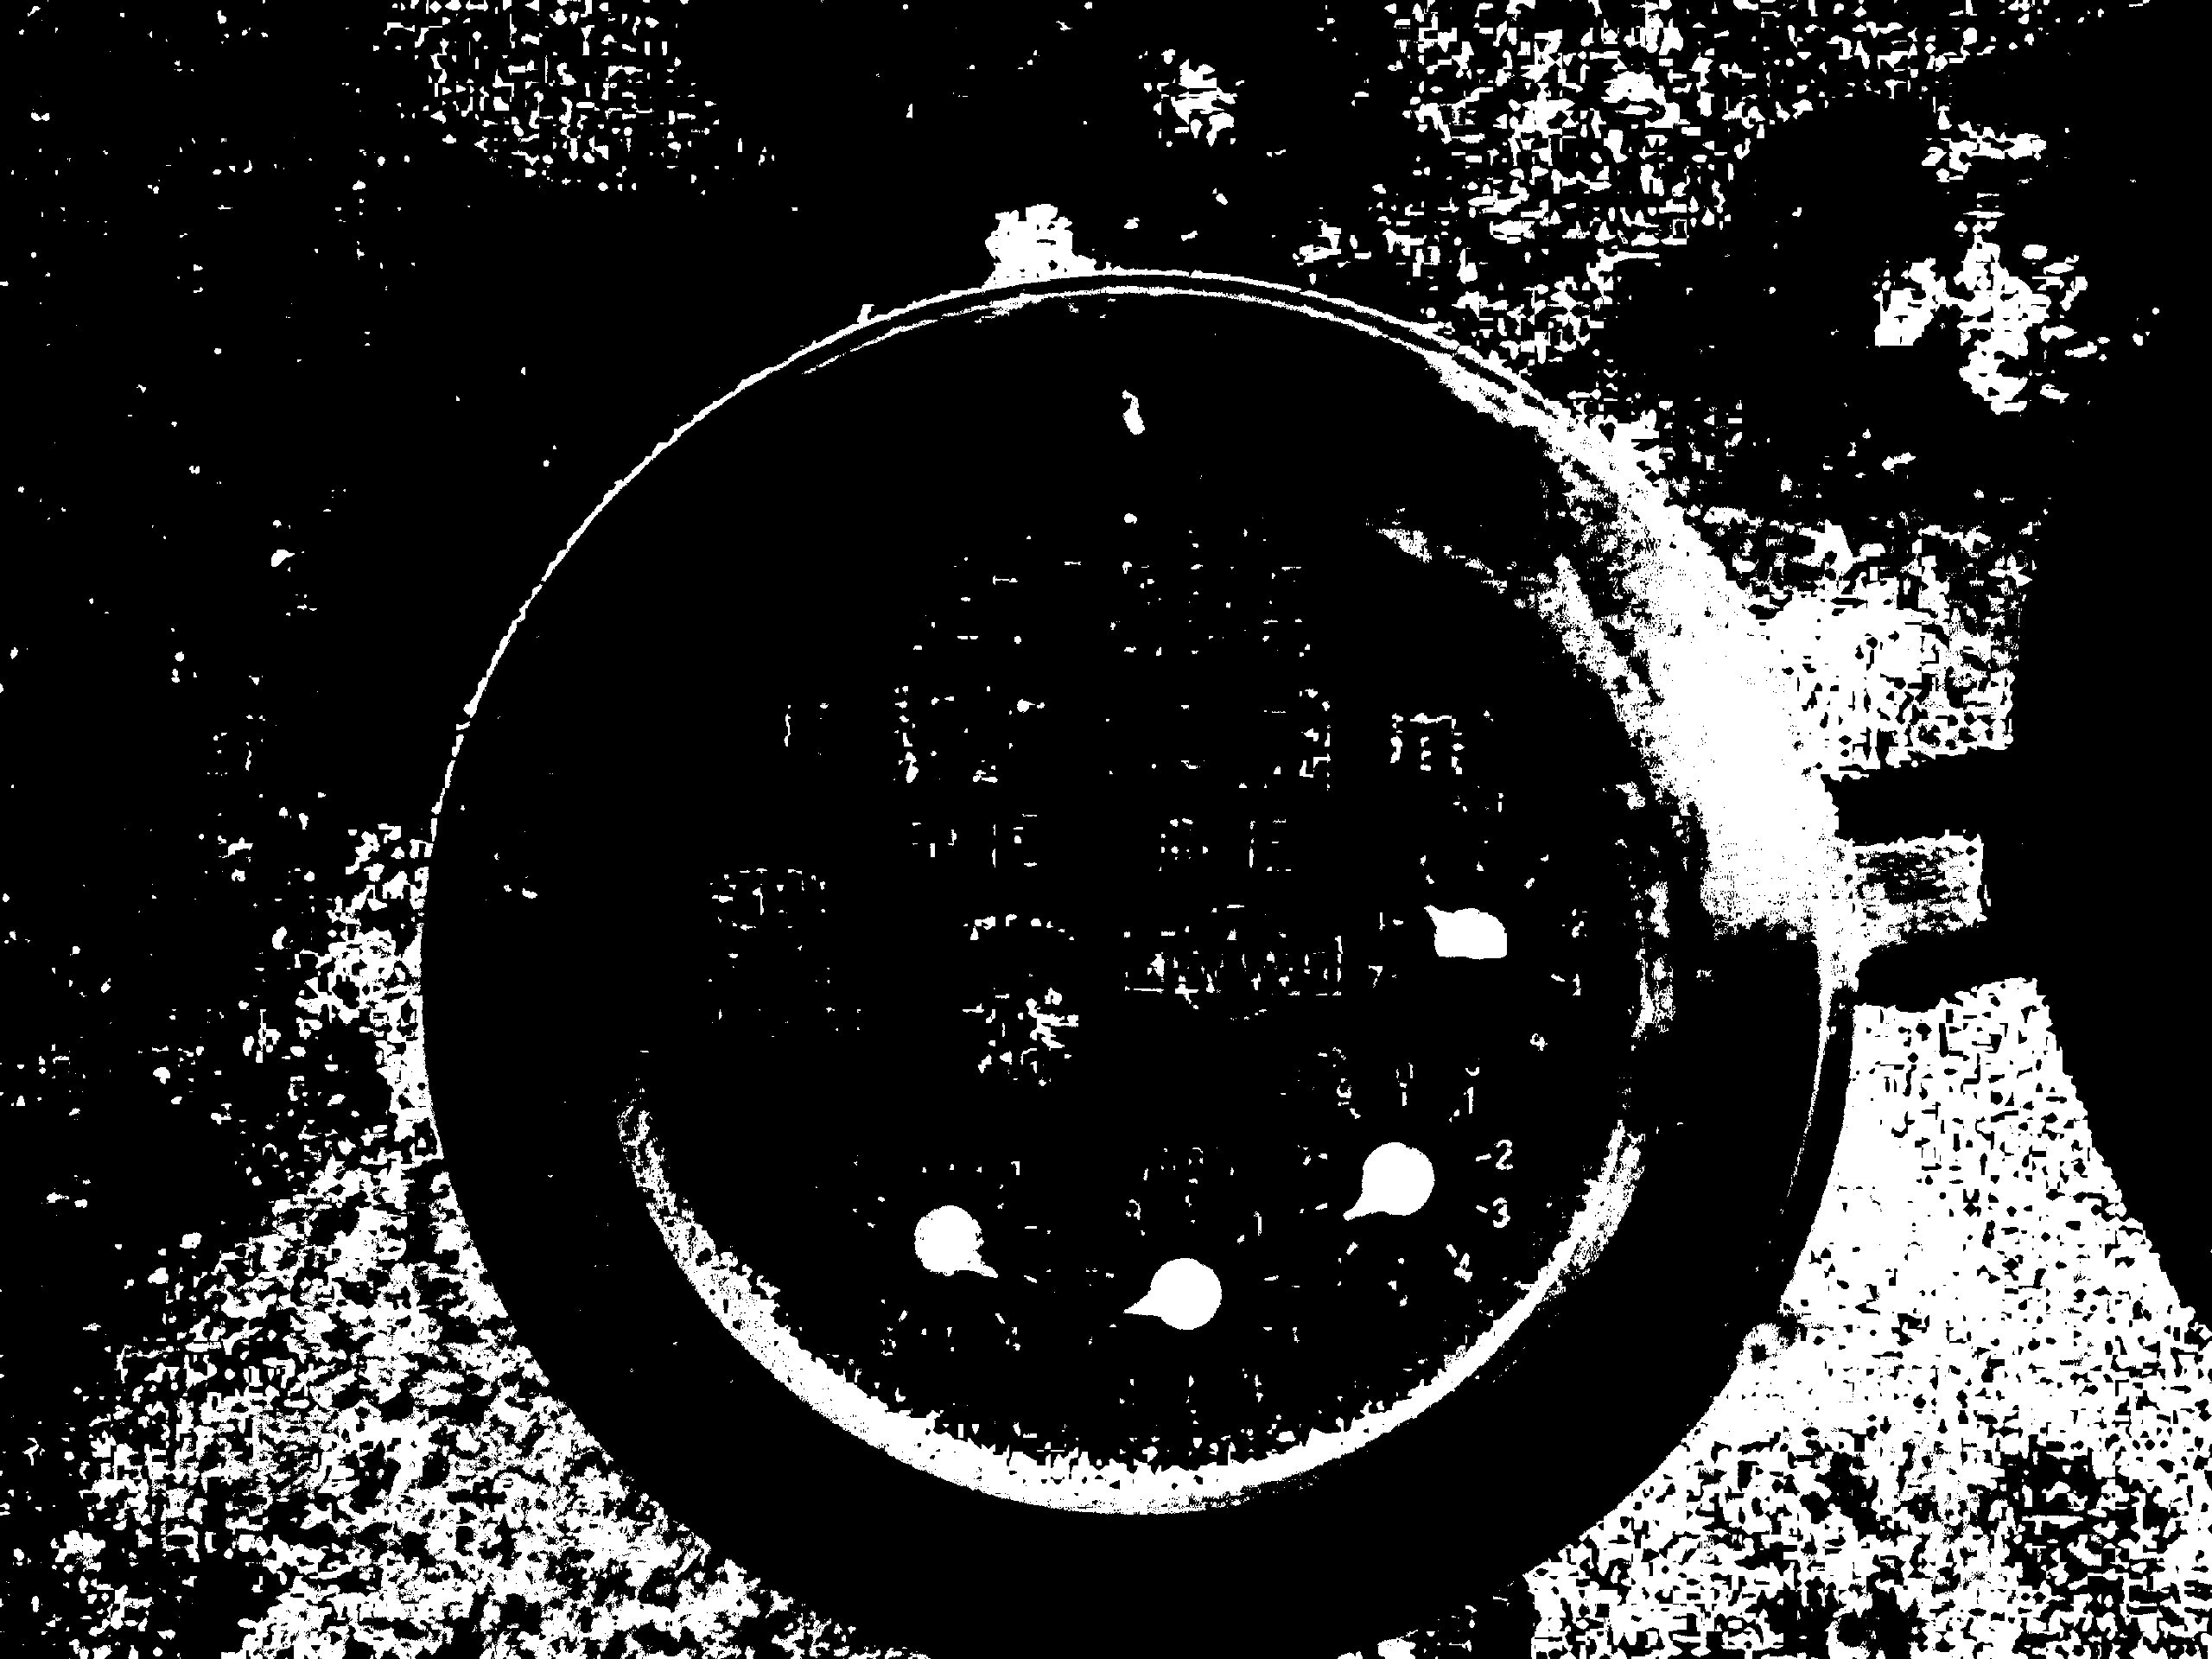
\includegraphics[width=\textwidth]{figure/threshold/img2.jpg}
	\end{minipage}\\
	\begin{minipage}[t]{0.25\textwidth}
		\centering
		
\includegraphics[width=\textwidth]{figure/threshold/img3.jpg}
	\end{minipage}
	\begin{minipage}[t]{0.25\textwidth}
		\centering
		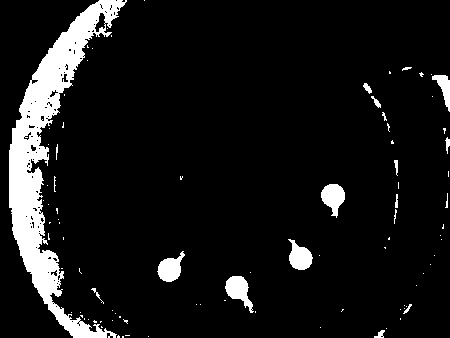
\includegraphics[width=\textwidth]{figure/threshold/img4.jpg}
	\end{minipage}
	\begin{minipage}[t]{0.25\textwidth}
		\centering
		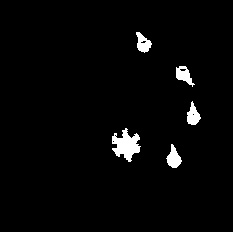
\includegraphics[width=\textwidth]{figure/threshold/img5.jpg}
	\end{minipage}
	\caption{阈值化处理结果}\label{fig:阈值化}
\end{figure}

\subsubsection{K聚类法}\label{sec:K聚类}
K聚类法\cite{chen2008fast}算法的核心思想是将n个数据对象划分成k个聚类,使每个聚类中的数据与该聚类中心距离的平方和最小,用K聚类算法对图像聚类是将图像中的每一个像素点作为一个样本,对其色彩进行聚类,从而达到分割图像的目的。
K聚类法可以用于提取黑色指针区域,选择聚类中心为4,取聚类结果的第一类(偏黑色的像素)作为黑色指针区域的划分结果,形成程序文件“kmeans.py”,对图像进行二值化分割处理,结果如图\ref{fig:K聚类}。

\begin{figure}[htbp]
	\centering
	\begin{minipage}[t]{0.25\textwidth}
		\centering
		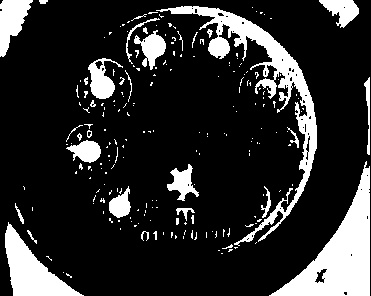
\includegraphics[width=\textwidth]{figure/kmeans/img1.jpg}
	\end{minipage}
	\begin{minipage}[t]{0.25\textwidth}
		\centering
		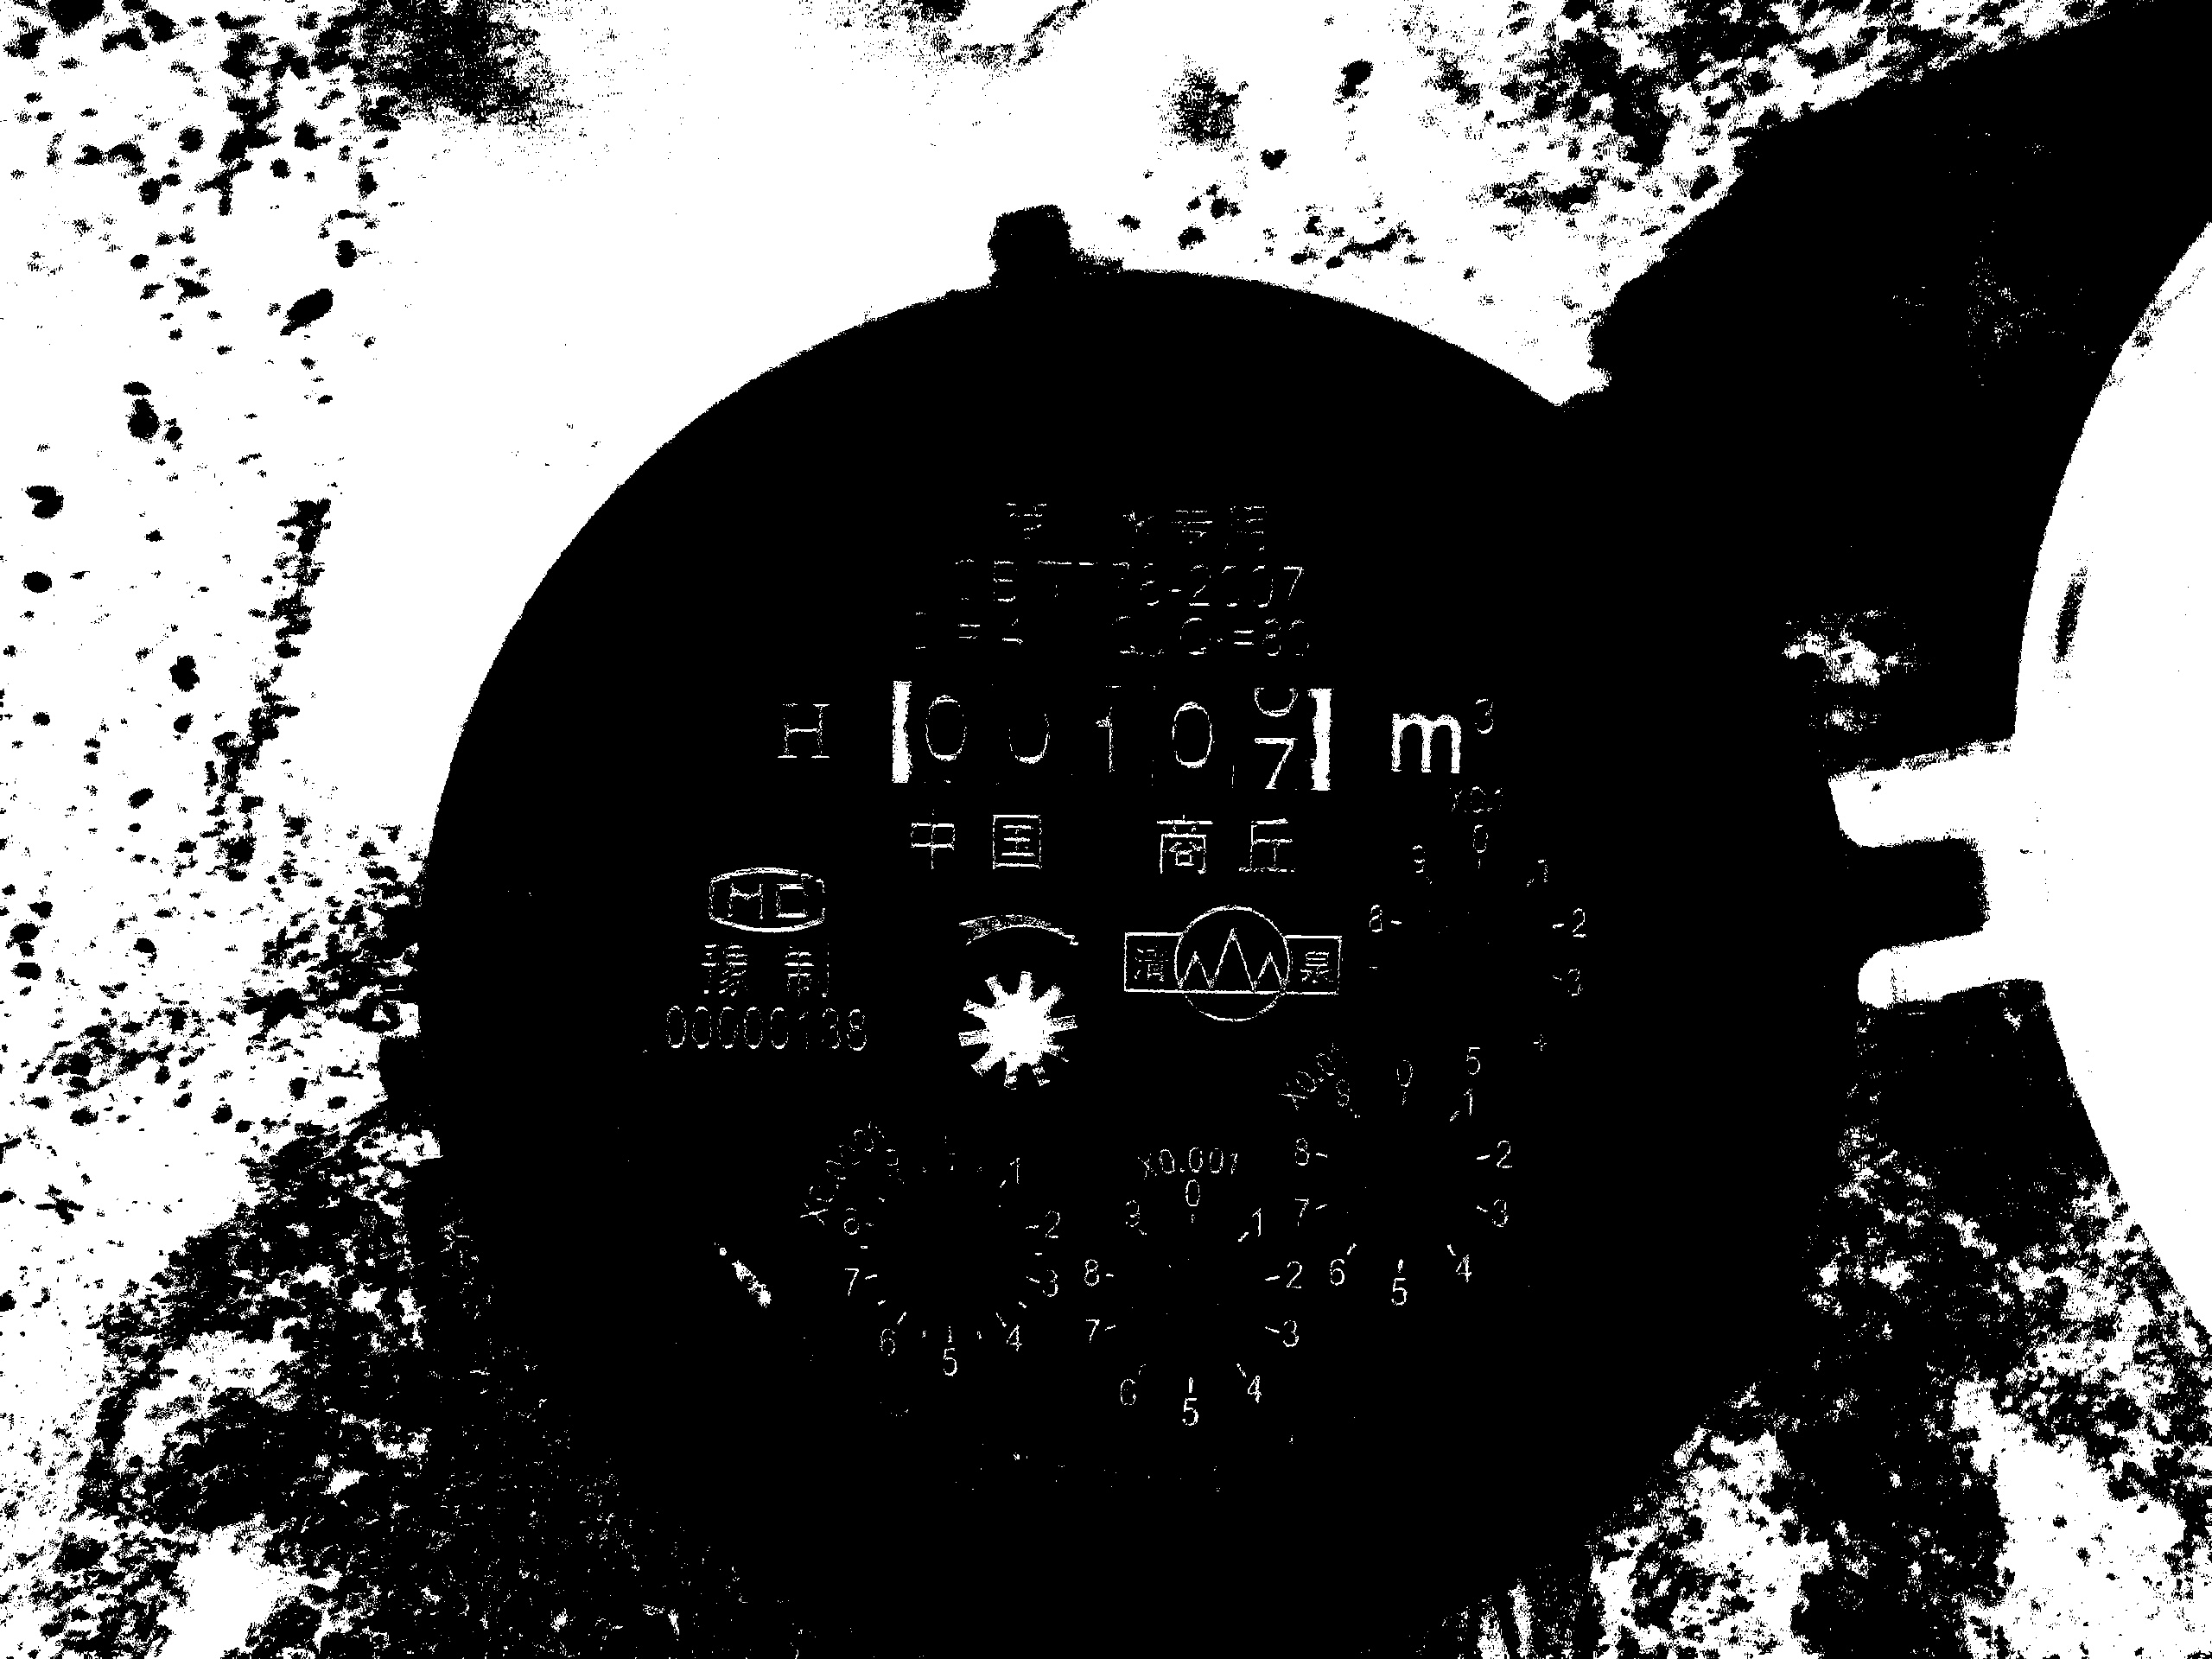
\includegraphics[width=\textwidth]{figure/kmeans/img2.jpg}
	\end{minipage}\\
	\begin{minipage}[t]{0.25\textwidth}
		\centering
		
\includegraphics[width=\textwidth]{figure/kmeans/img3.jpg}
	\end{minipage}
	\begin{minipage}[t]{0.25\textwidth}
		\centering
		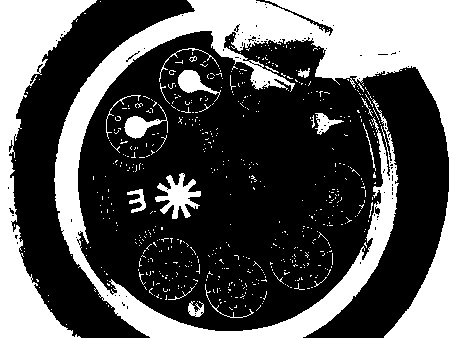
\includegraphics[width=\textwidth]{figure/kmeans/img4.jpg}
	\end{minipage}
	\begin{minipage}[t]{0.25\textwidth}
		\centering
		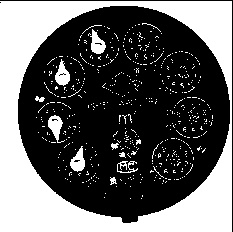
\includegraphics[width=\textwidth]{figure/kmeans/img5.jpg}
	\end{minipage}
	\caption{K聚类处理结果}\label{fig:K聚类}
\end{figure}

\subsubsection{形态学处理}
在\ref{sec:阈值化}节和\ref{sec:K聚类}节中得到的划分结果显然不能直接用于判定指针方向,需要进行进一步的形态学处理:

\begin{enumerate}[label=\arabic*、]
	\item 分离指针:划分结果图\ref{fig:阈值化}和图\ref{fig:K聚类}中均有很多非目标部分与指针区域相连,需要使用开操作将指针区域与非指针区域进行分离。步骤如下:
	\begin{enumerate}[label=\alph*)]
		\item 选择边长为图片高度$\div$200的方形核对图\ref{fig:阈值化}中的结果进行一次开运算、一次膨胀、一次开运算、四次膨胀、四次腐蚀操作分离指针区域,结果如图\ref{fig:阈值化开运算};
		\begin{figure}[htbp]
			\centering
			\begin{minipage}[t]{0.25\textwidth}
				\centering
				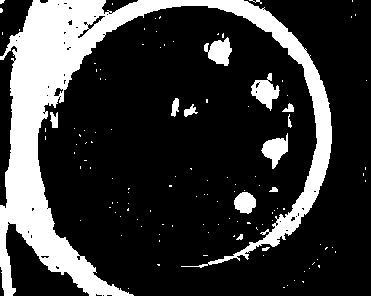
\includegraphics[width=\textwidth]{figure/open_1/img1.jpg}
			\end{minipage}
			\begin{minipage}[t]{0.25\textwidth}
				\centering
				
\includegraphics[width=\textwidth]{figure/open_1/img2.jpg}
			\end{minipage}\\
			\begin{minipage}[t]{0.25\textwidth}
				\centering
				
\includegraphics[width=\textwidth]{figure/open_1/img3.jpg}
			\end{minipage}
			\begin{minipage}[t]{0.25\textwidth}
				\centering
				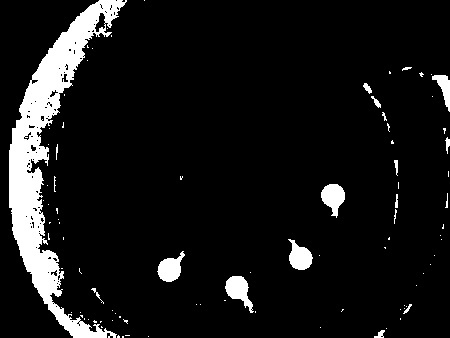
\includegraphics[width=\textwidth]{figure/open_1/img4.jpg}
			\end{minipage}
			\begin{minipage}[t]{0.25\textwidth}
				\centering
				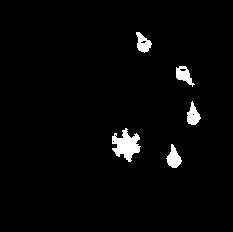
\includegraphics[width=\textwidth]{figure/open_1/img5.jpg}
			\end{minipage}
			\caption{阈值化处理开运算结果}\label{fig:阈值化开运算}
		\end{figure}
		
		\item 选择边长为图片高度$\div$110的方形核对图\ref{fig:K聚类}中的结果进行三次开操作分离指针,结果如图\ref{fig:K聚类开运算}。
		\begin{figure}[htbp]
			\centering
			\begin{minipage}[t]{0.25\textwidth}
				\centering
				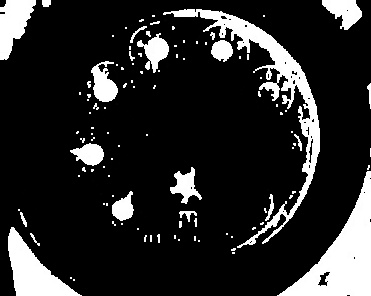
\includegraphics[width=\textwidth]{figure/open_2/img1.jpg}
			\end{minipage}
			\begin{minipage}[t]{0.25\textwidth}
				\centering
				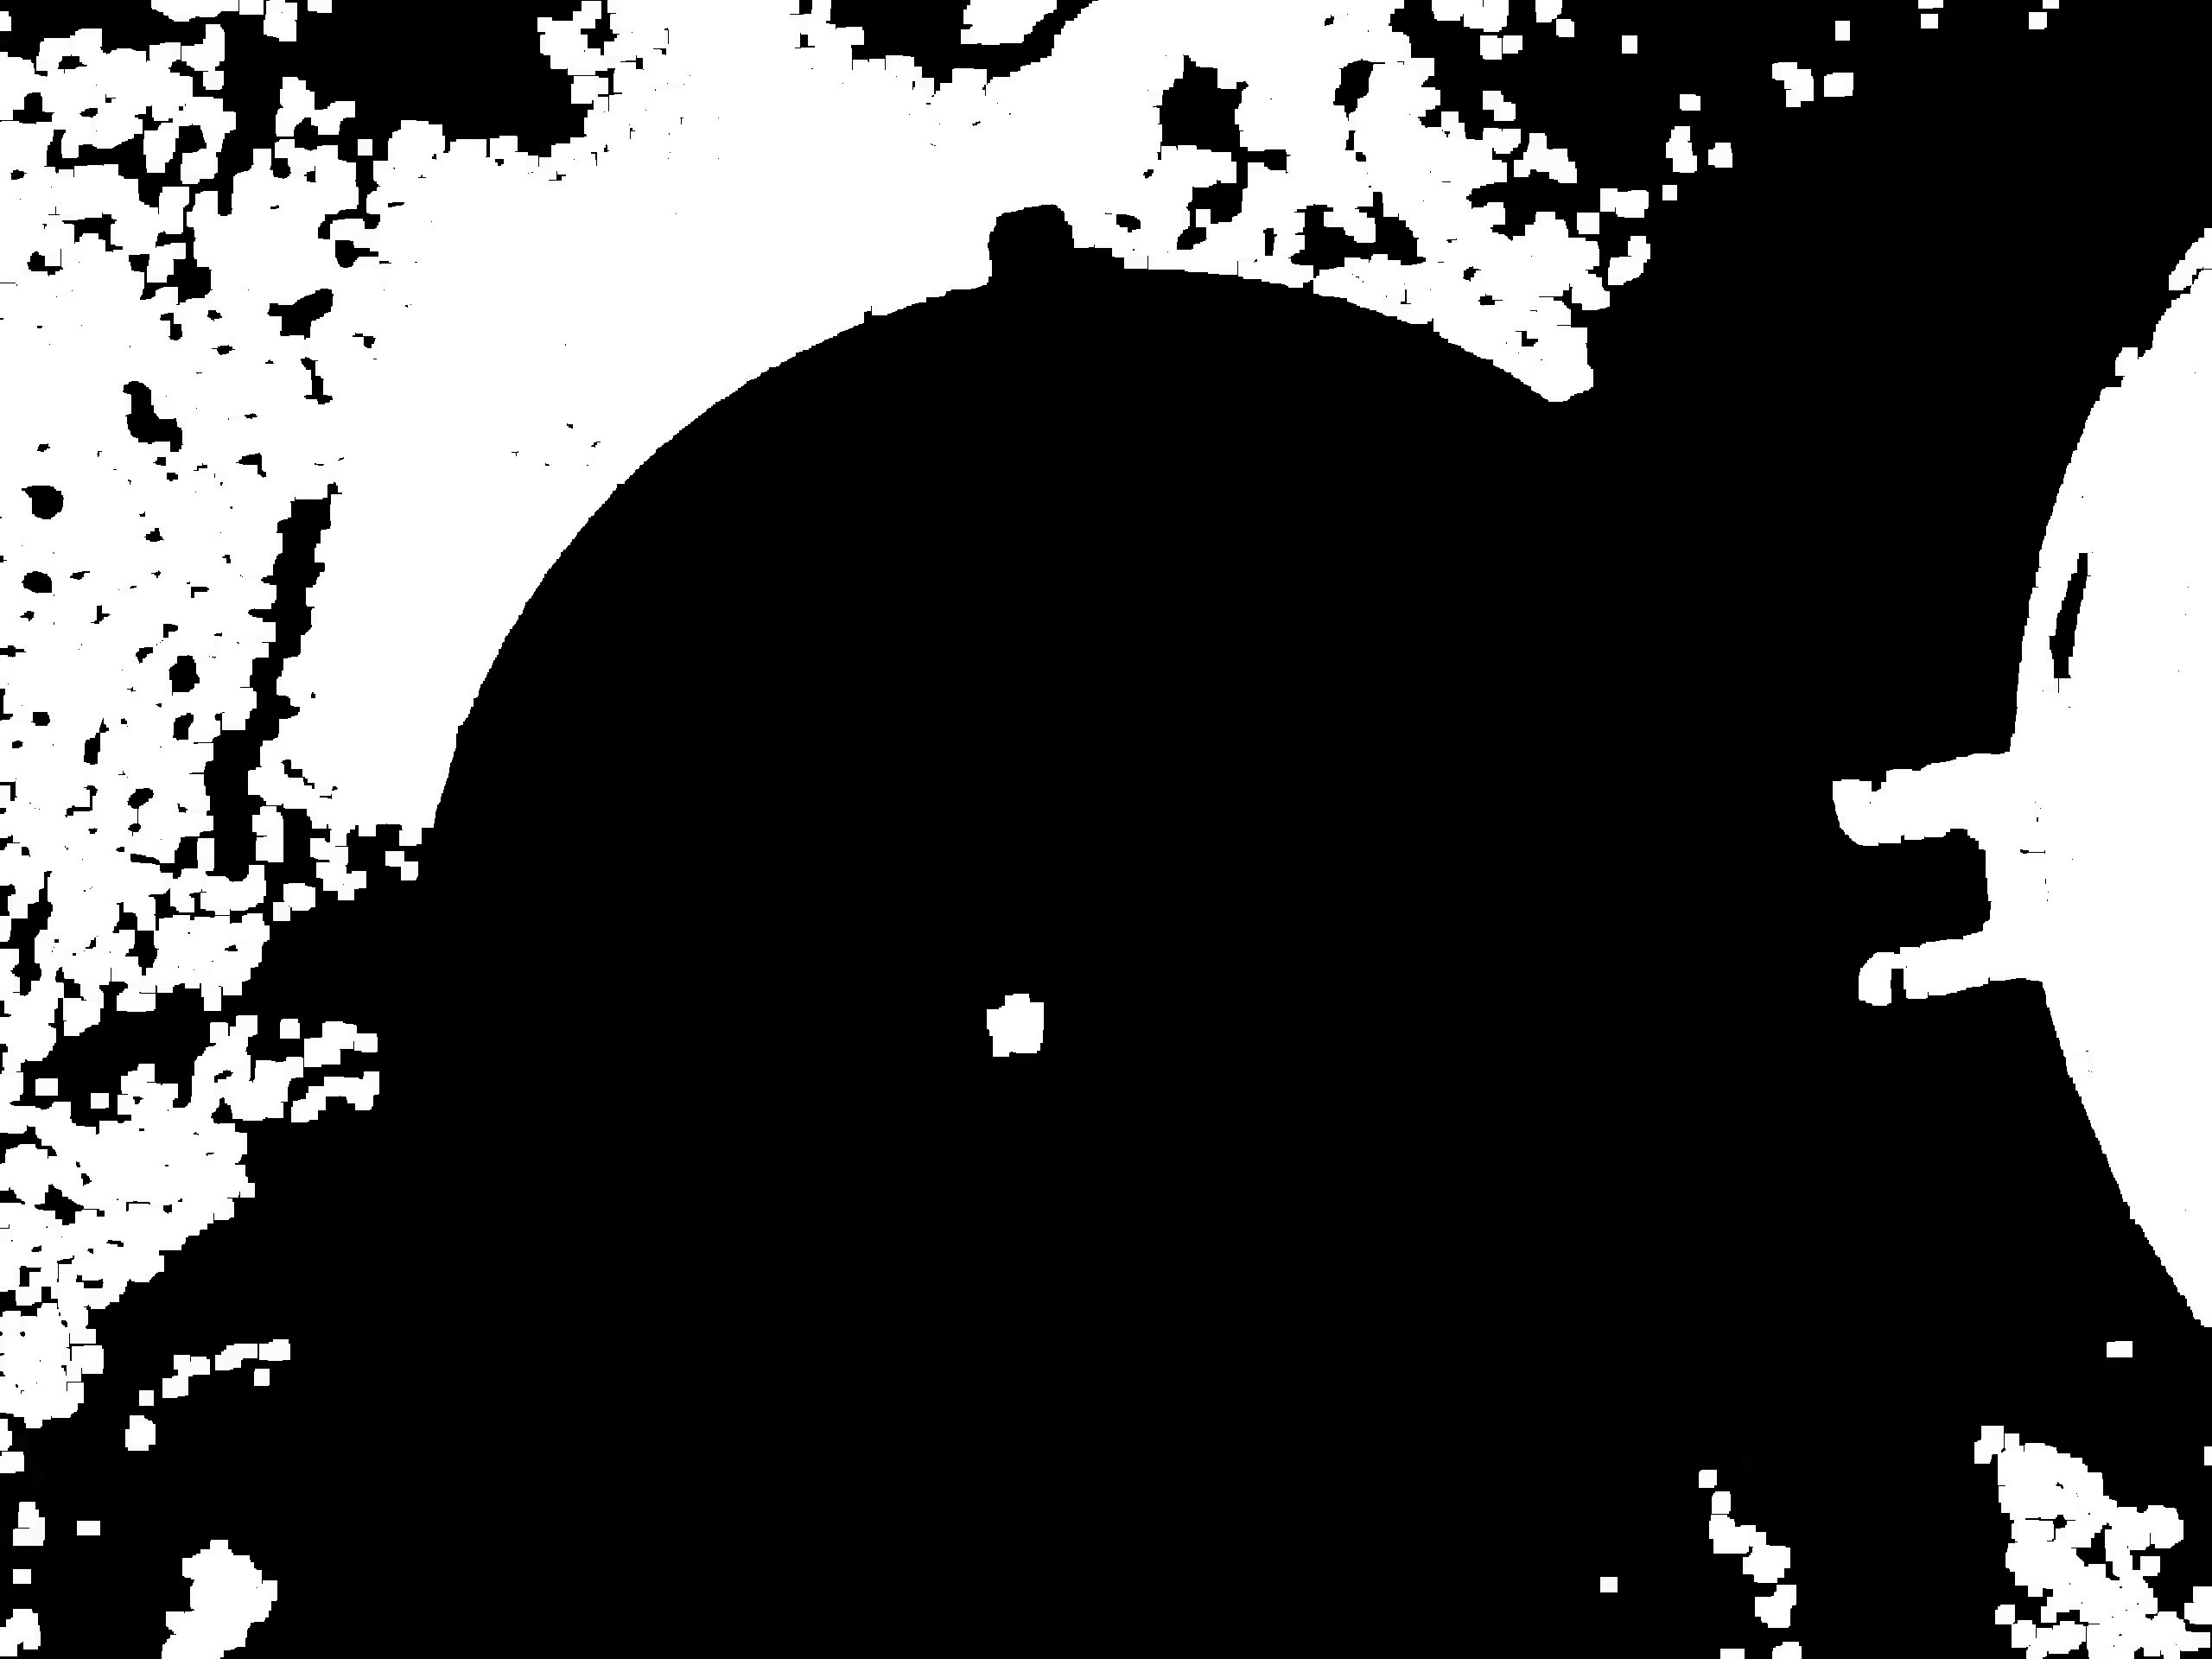
\includegraphics[width=\textwidth]{figure/open_2/img2.jpg}
			\end{minipage}\\
			\begin{minipage}[t]{0.25\textwidth}
				\centering
				
\includegraphics[width=\textwidth]{figure/open_2/img3.jpg}
			\end{minipage}
			\begin{minipage}[t]{0.25\textwidth}
				\centering
				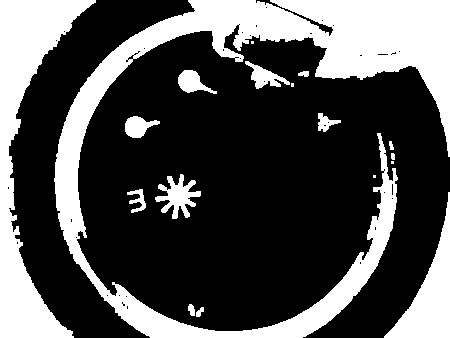
\includegraphics[width=\textwidth]{figure/open_2/img4.jpg}
			\end{minipage}
			\begin{minipage}[t]{0.25\textwidth}
				\centering
				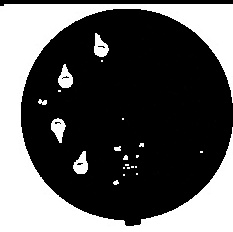
\includegraphics[width=\textwidth]{figure/open_2/img5.jpg}
			\end{minipage}
			\caption{K聚类处理开运算结果}\label{fig:K聚类开运算}
		\end{figure}
	\end{enumerate}
	
	\item 区域筛选:由图\ref{fig:阈值化开运算}和图\ref{fig:K聚类开运算}的结果可以看出,开运算成功的将指针的主要区域和无关区域分离开来,这时就可以通过提取图像中各连通域的大小,删去面积过大的背景区域和面积过小噪点区域,而只留下面积适中的指针区域,步骤如下:
	\begin{enumerate}[label=\alph*)]
		\item 使用cv2.connectedComponentsWithStats函数提取图\ref{fig:阈值化开运算}中的4连通区域,选择面积阈值范围为图像面积/400$\sim$图像面积/150,保留面积在面积阈值范围内的连通区域,即可提取出红色指针区域,结果如图\ref{fig:阈值化开运算区域选择},图中不同灰度表示不同的连通区域;
		\begin{figure}[htbp]
			\centering
			\begin{minipage}[t]{0.25\textwidth}
				\centering
				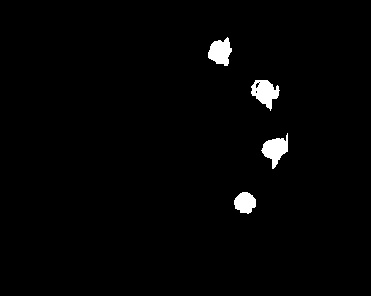
\includegraphics[width=\textwidth]{figure/drop_1/img1.jpg}
			\end{minipage}
			\begin{minipage}[t]{0.25\textwidth}
				\centering
				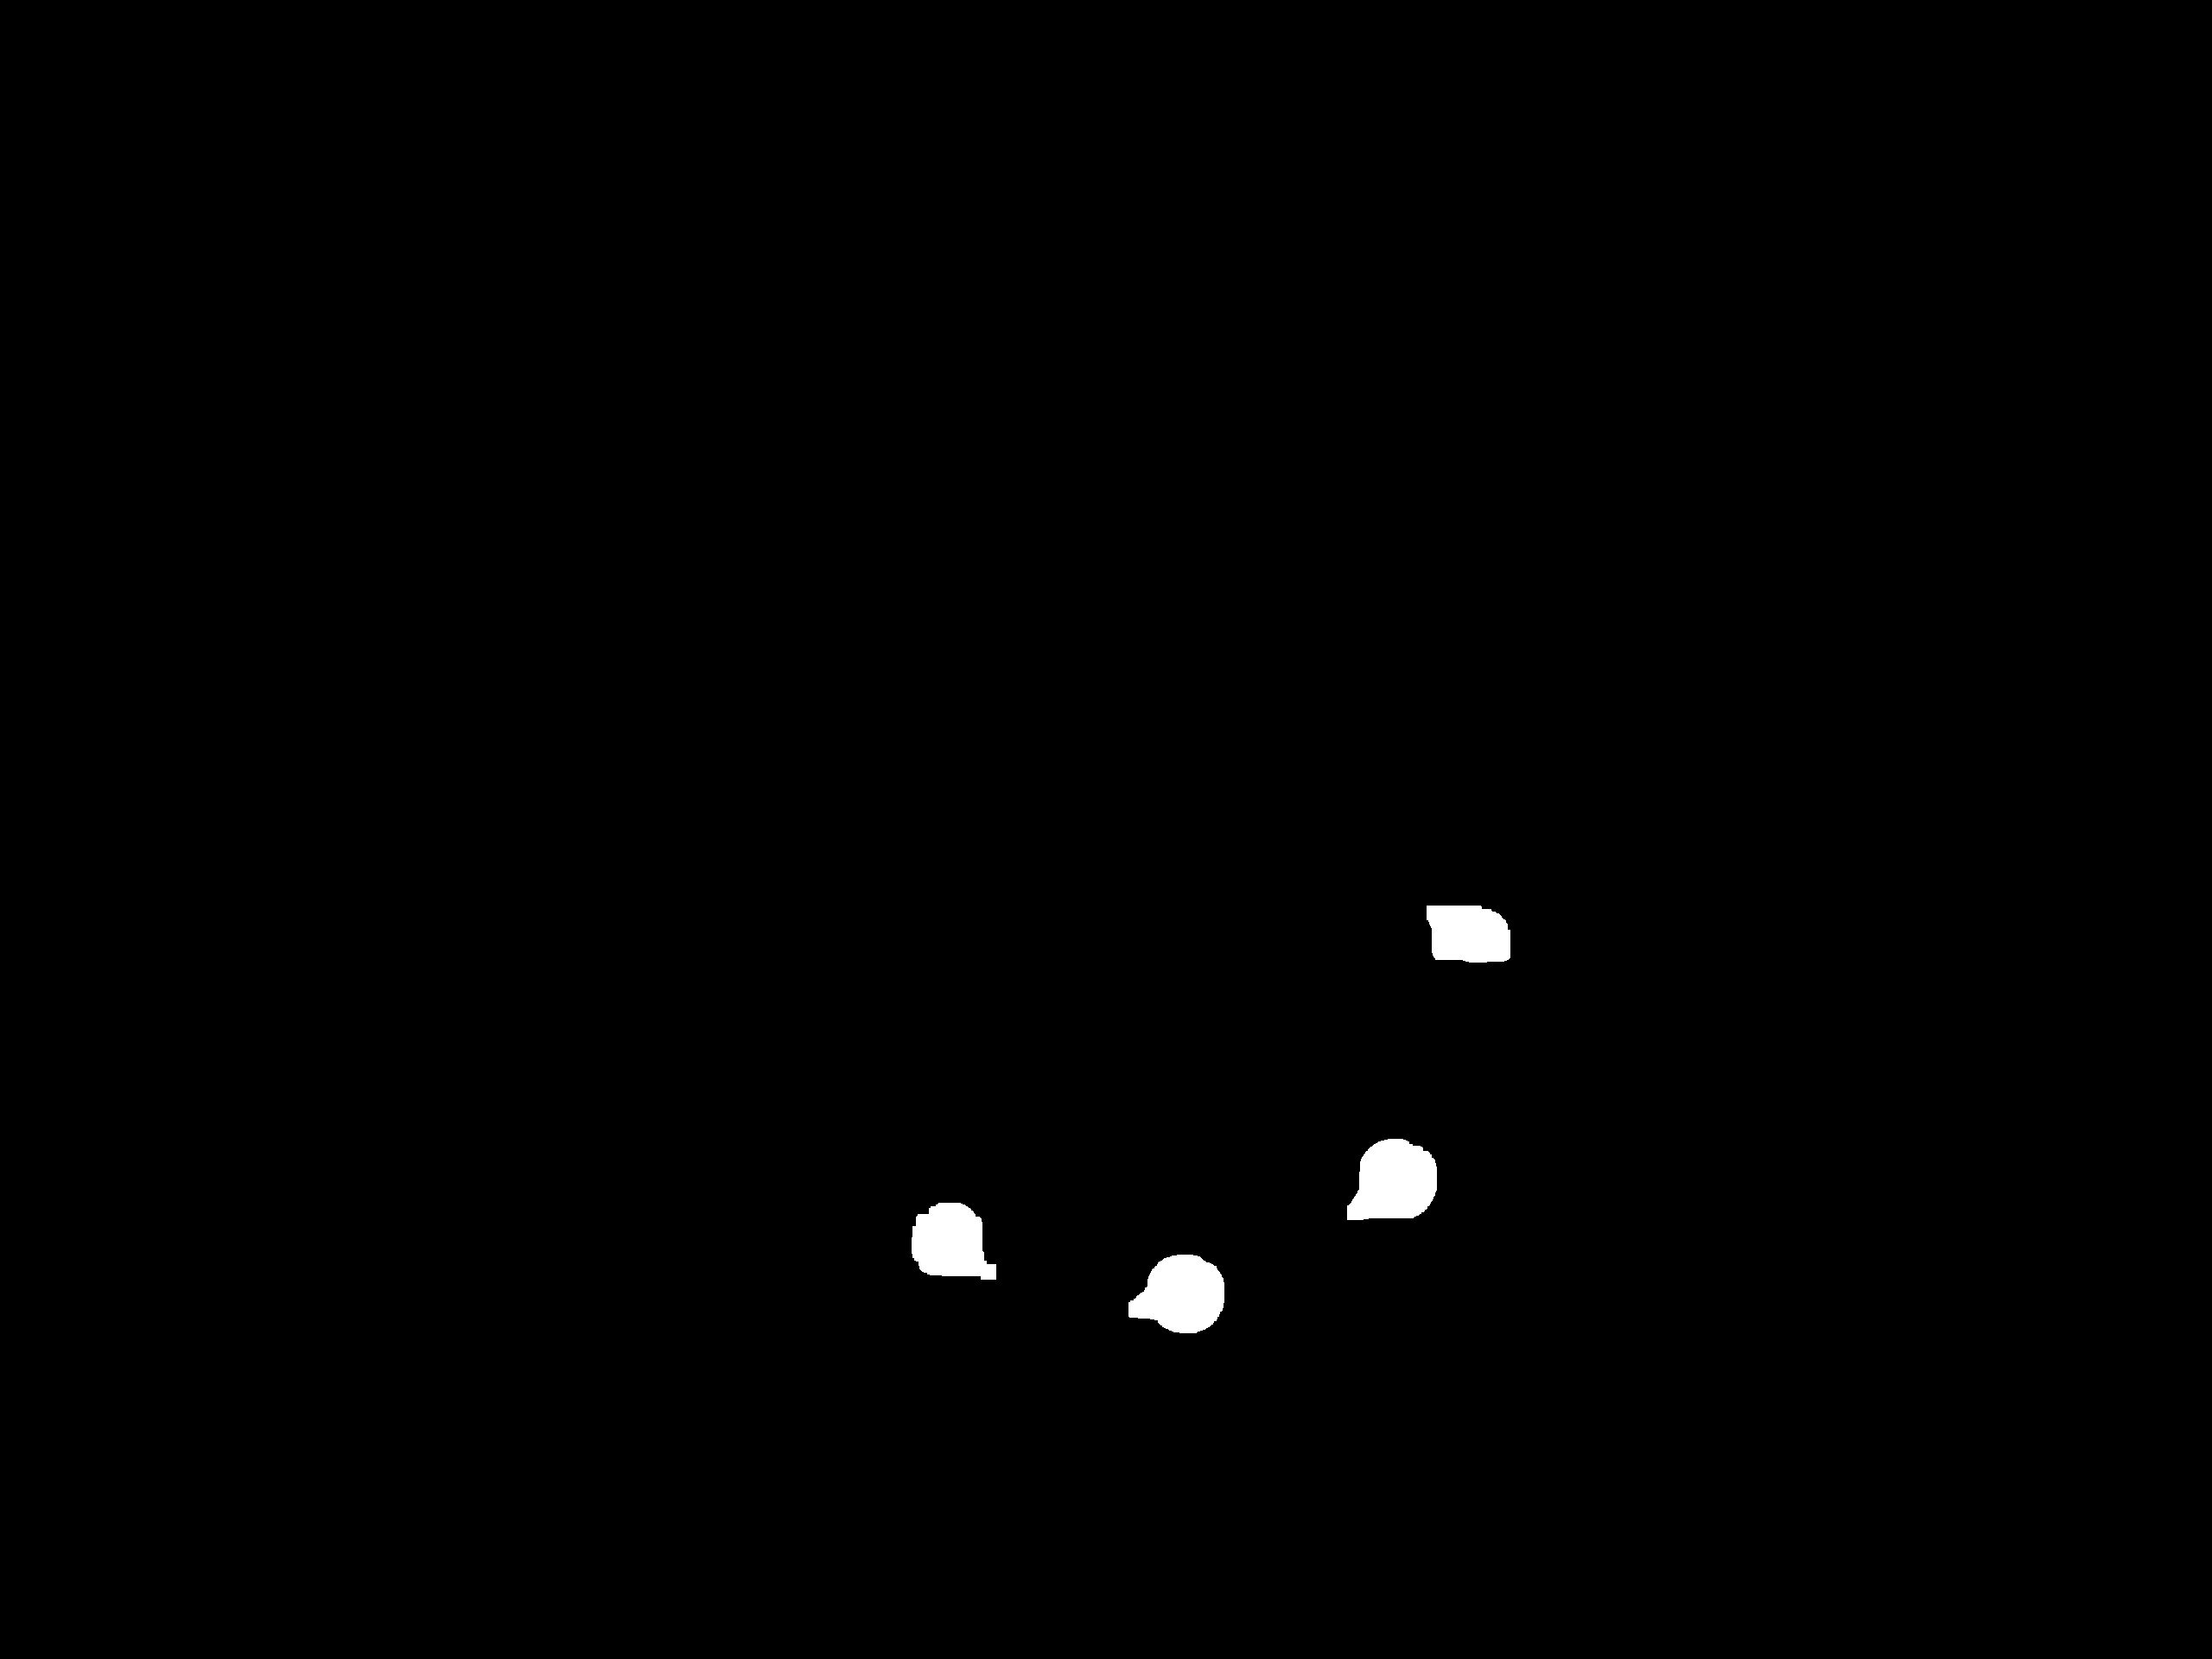
\includegraphics[width=\textwidth]{figure/drop_1/img2.jpg}
			\end{minipage}\\
			\begin{minipage}[t]{0.25\textwidth}
				\centering
				
\includegraphics[width=\textwidth]{figure/drop_1/img3.jpg}
			\end{minipage}
			\begin{minipage}[t]{0.25\textwidth}
				\centering
				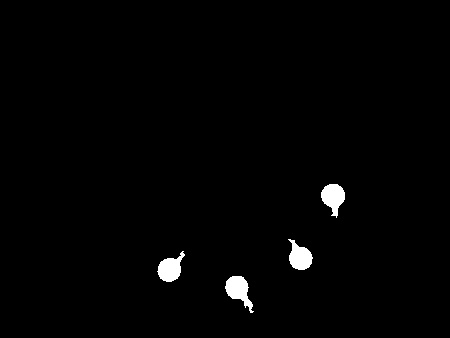
\includegraphics[width=\textwidth]{figure/drop_1/img4.jpg}
			\end{minipage}
			\begin{minipage}[t]{0.25\textwidth}
				\centering
				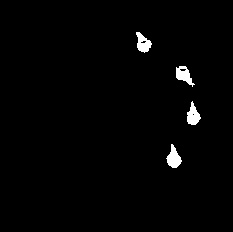
\includegraphics[width=\textwidth]{figure/drop_1/img5.jpg}
			\end{minipage}
			\caption{阈值化处理开运算区域选择结果}\label{fig:阈值化开运算区域选择}
		\end{figure}
		
		\item 使用cv2.connectedComponentsWithStats函数提取图\ref{fig:K聚类开运算}的4连通区域,选择面积阈值范围为图像面积/400$\sim$图像面积/150,保留面积在面积阈值范围内的连通区域,即可提取出黑色指针区域,结果如图\ref{fig:阈值化开运算区域选择},图中不同灰度表示不同的连通区域。
		\begin{figure}[htbp]
			\centering
			\begin{minipage}[t]{0.25\textwidth}
				\centering
				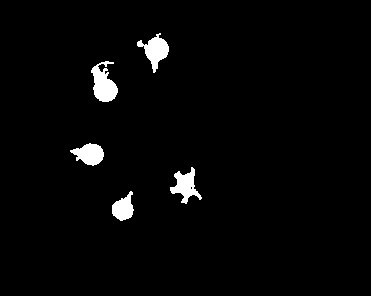
\includegraphics[width=\textwidth]{figure/drop_2/img1.jpg}
			\end{minipage}
			\begin{minipage}[t]{0.25\textwidth}
				\centering
				
\includegraphics[width=\textwidth]{figure/drop_2/img2.jpg}
			\end{minipage}\\
			\begin{minipage}[t]{0.25\textwidth}
				\centering
				
\includegraphics[width=\textwidth]{figure/drop_2/img3.jpg}
			\end{minipage}
			\begin{minipage}[t]{0.25\textwidth}
				\centering
				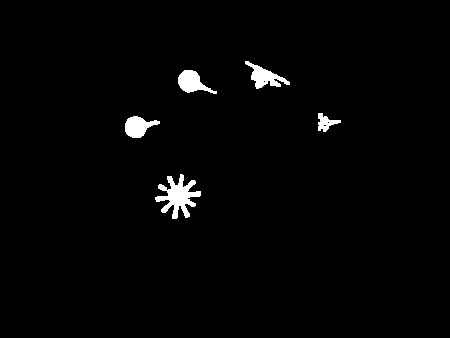
\includegraphics[width=\textwidth]{figure/drop_2/img4.jpg}
			\end{minipage}
			\begin{minipage}[t]{0.25\textwidth}
				\centering
				\includegraphics[width=\textwidth]{figure/drop_2/img5.jpg}
			\end{minipage}
			\caption{K聚类处理开运算区域选择结果}\label{fig:K聚类开运算区域选择}
		\end{figure}
	\end{enumerate}
	
	\item 图片拼合:将上一步中区域筛选的结果进行拼合,以使得红色指针区域和黑色指针区域显示在同一张图片上,结果如图\ref{fig:图片拼合}。
	\begin{figure}[htbp]
		\centering
		\begin{minipage}[t]{0.25\textwidth}
			\centering
			\includegraphics[width=\textwidth]{figure/add/img1.jpg}
		\end{minipage}
		\begin{minipage}[t]{0.25\textwidth}
			\centering
			\includegraphics[width=\textwidth]{figure/add/img2.jpg}
		\end{minipage}\\
		\begin{minipage}[t]{0.25\textwidth}
			\centering
			\includegraphics[width=\textwidth]{figure/add/img3.jpg}
		\end{minipage}
		\begin{minipage}[t]{0.25\textwidth}
			\centering
			\includegraphics[width=\textwidth]{figure/add/img4.jpg}
		\end{minipage}
		\begin{minipage}[t]{0.25\textwidth}
			\centering
			\includegraphics[width=\textwidth]{figure/add/img5.jpg}
		\end{minipage}
		\caption{图片拼合结果}\label{fig:图片拼合}
	\end{figure}
	\item 进一步的区域筛选:在图\ref{fig:图片拼合}所示的结果中,仍包含部分非指针区域,需要进行进一步的剔除。观察发现,图\ref{fig:图片拼合}所示结果中的非指针区域都是靠近标牌中心的叶轮齿,可以通过区域位置加以筛除,具体流程如算法\ref{alg:1}所示。
	\begin{algorithm}
		\caption{基于质心位置的区域筛选法}
		\label{alg:1}
		\begin{algorithmic}[1]
			\Require $\bm I\gets$读入图像
			\State $\mathcal A\gets$分割图像$\bm I$的连通区域
			\If{连通区域数量$|\mathcal A|>8$}
			\State $\bm p\gets$求$\mathcal A$中所有区域的质心
			\State 删除与$\bm p$点质心距离最近的连通区域
			\EndIf
		\end{algorithmic}
	\end{algorithm}
	其结果如图\ref{fig:进一步筛选结果},图中不同灰度表示不同的连通区域。
	\begin{figure}[htbp]
		\centering
		\begin{minipage}[t]{0.25\textwidth}
			\centering
			\includegraphics[width=\textwidth]{figure/drop_center/img1.jpg}
		\end{minipage}
		\begin{minipage}[t]{0.25\textwidth}
			\centering
			\includegraphics[width=\textwidth]{figure/drop_center/img2.jpg}
		\end{minipage}\\
		\begin{minipage}[t]{0.25\textwidth}
			\centering
			\includegraphics[width=\textwidth]{figure/drop_center/img3.jpg}
		\end{minipage}
		\begin{minipage}[t]{0.25\textwidth}
			\centering
			\includegraphics[width=\textwidth]{figure/drop_center/img4.jpg}
		\end{minipage}
		\begin{minipage}[t]{0.25\textwidth}
			\centering
			\includegraphics[width=\textwidth]{figure/drop_center/img5.jpg}
		\end{minipage}
		\caption{进一步区域筛选结果}\label{fig:进一步筛选结果}
	\end{figure}
\end{enumerate}
\newpage

\subsection{指针读数}
当所有的指针区域都被分割出来后,就可以进行指针读数了。考虑到图中各表盘都有偏转,因此除判定指针与水平方向的夹角$\theta_{\text{指针}}$外,还需要判定表盘与水平方向的夹角$\theta_{\text{表盘}}$,最终求出指针相对于表盘水平方向的夹角$\theta=\theta_{\text{指针}}-\theta_{\text{表盘}}$用于读数判定。

\subsubsection{判定指针与水平方向的夹角}\label{sec:1}
判定指针方向可以通过求连通域内相距最远的两点所连成的直线与水平方向的夹角而求得,具体流程如算法\ref{alg:2}所示,其结果如图\ref{fig:进一步筛选结果},表盘所指方向及与水平方向夹角已标出。
\begin{algorithm}
	\caption{判定指针与水平方向的夹角}
	\label{alg:2}
	\begin{algorithmic}[1]
		\Require $\bm I\gets$读入图像
		\State $\mathcal A\gets$图像$I$的连通区域
		\For{$\mathcal A$中的每个连通区域$\bm A_i$}
		\State $\bm p_{\text{指针}i}\gets$连通区域$\bm A_i$的质心
		\State $\bm p_1,\bm p_2\gets\bm A_i$中相距最远的两点
		\If{$|\bm p_{\text{指针}i}-\bm p_1|>|\bm p_{\text{指针}i}-\bm p_2|$}
		\State $\theta_{\text{指针}i}\gets arg(\bm p_1-\bm p_2)$
		\Else
		\State $\theta_{\text{指针}i}\gets arg(\bm p_2-\bm p_1)$
		\EndIf
		\EndFor
		\Ensure $\Theta=\left\{(\bm p_{\text{指针}i},\theta_{\text{指针}i})\right\}$
	\end{algorithmic}
\end{algorithm}
\begin{figure}[htbp]
	\centering
	\begin{minipage}[t]{0.25\textwidth}
		\centering
		\includegraphics[width=\textwidth]{figure/point_to/img1.jpg}
	\end{minipage}
	\begin{minipage}[t]{0.25\textwidth}
		\centering
		\includegraphics[width=\textwidth]{figure/point_to/img2.jpg}
	\end{minipage}\\
	\begin{minipage}[t]{0.25\textwidth}
		\centering
		\includegraphics[width=\textwidth]{figure/point_to/img3.jpg}
	\end{minipage}
	\begin{minipage}[t]{0.25\textwidth}
		\centering
		\includegraphics[width=\textwidth]{figure/point_to/img4.jpg}
	\end{minipage}
	\begin{minipage}[t]{0.25\textwidth}
		\centering
		\includegraphics[width=\textwidth]{figure/point_to/img5.jpg}
	\end{minipage}
	\caption{进一步区域筛选结果}\label{fig:进一步筛选结果}
\end{figure}

\subsubsection{判定表盘与水平方向的夹角}\label{sec:2}
本实验中所涉及的表盘有两种,一种是有8个指针的表盘,一种是有4个指针的表盘,针对这两种表盘,需要采用不同的方法进行处理:
\begin{itemize}
	\item 针对8指针表盘:在8指针表盘中,表盘指针位置关于表盘中轴线对称且除在表盘最底部的两个指针外,其余指针相互之间夹角相同,因此可以通过8个指针的质心与指针各自的质心之间的连线夹角判定表盘方向,即当相邻指针间的连续夹角大于某一阈值时,可以判断表盘中轴即为这两个指针连线中点与质心的连线;
	\item 针对4指针表盘:在4指针表盘中,表盘的水平方向是表盘圆心与顺时针方向第一个指针间的连线方向,该连线与即是表盘与水平方向的夹角。
\end{itemize}
依据上述思路编写程序,形成程序文件“bias.py”,对\ref{fig:进一步筛选结果}中的结果进行表盘与水平方向夹角的判定,结果如表\ref{tbl:表盘与水平方向夹角}。
\begin{table}
	\centering
	\caption{表盘与水平方向夹角}\label{tbl:表盘与水平方向夹角}
	\begin{tabular}{|c|c|}
		\hline
		图片&偏离角度\\
		\hline
		图\ref{fig:1}&$0.7489^\circ$\\
		图\ref{fig:2}&$-6.1157^\circ$\\
		图\ref{fig:3}&$-19.6311^\circ$\\
		图\ref{fig:4}&$-78.1445^\circ$\\
		图\ref{fig:5}&$-1.5154^\circ$\\
		\hline
	\end{tabular}
\end{table}

\subsubsection{读取表盘指针角度}
由\ref{sec:1}节和\ref{sec:1}节的结论可以得到各表盘的指针实际偏转角度(顺时针方向数指针,以水平方向为$0^\circ$。
\begin{itemize}
	\item 图\ref{fig:1}中的指针角度:$68.4711^\circ$、$168.8511^\circ$、$73.4911^\circ$、$-100.7489^\circ$、$66.3111^\circ$、$62.6511^\circ$、$66.0511^\circ$、$23.4711^\circ$;
	\item 图\ref{fig:2}中的指针角度:$181.0157^\circ$、$148.1157^\circ$、$164.1157^\circ$、$-33.6843^\circ$;
	\item 图\ref{fig:3}中的指针角度:$30.0111^\circ$、$179.8311^\circ$、$-96.3689^\circ$、$-167.3311^\circ$;
	\item 图\ref{fig:4}中的指针角度:$94.5245^\circ$、$55.3445^\circ$、$50.6445^\circ$、$102.5845^\circ$、$0.1445^\circ$、$203.6445^\circ$、$20.3445^\circ$、$127.7145^\circ$;
	\item 图\ref{fig:5}中的指针角度:$71.5254^\circ$、$-78.9846^\circ$、$101.3754^\circ$、$110.6154^\circ$、$121.5154^\circ$、$-48.2846^\circ$、$98.9454^\circ$、$103.7154^\circ$。
\end{itemize}


\section{实验结果分析}
经过人工测量比对,图\ref{fig:1}和图\ref{fig:4}中有部分指针的程序测量结果和实际差距较大,而观察原图可以看出,这两张图中所示的水表指针较细且透明度较高,尤其是有部分红色指针的针尖部分几乎和背景融为一体难以区分,并且本文所使用的MSRCR色彩增强方法对这类比较透明的指针没有显著效果,因此造成程序识别效果不好,因此相比这两种水表,图\ref{fig:2}、图\ref{fig:4}和图\ref{fig:5}中所示的水表更适合用于构建基于机器视觉的自动抄表系统。

\bibliography{ref}
\end{document}